\documentclass[12pt]{article}\usepackage[]{graphicx}\usepackage[]{color}
% maxwidth is the original width if it is less than linewidth
% otherwise use linewidth (to make sure the graphics do not exceed the margin)
\makeatletter
\def\maxwidth{ %
  \ifdim\Gin@nat@width>\linewidth
    \linewidth
  \else
    \Gin@nat@width
  \fi
}
\makeatother

\definecolor{fgcolor}{rgb}{0.345, 0.345, 0.345}
\newcommand{\hlnum}[1]{\textcolor[rgb]{0.686,0.059,0.569}{#1}}%
\newcommand{\hlstr}[1]{\textcolor[rgb]{0.192,0.494,0.8}{#1}}%
\newcommand{\hlcom}[1]{\textcolor[rgb]{0.678,0.584,0.686}{\textit{#1}}}%
\newcommand{\hlopt}[1]{\textcolor[rgb]{0,0,0}{#1}}%
\newcommand{\hlstd}[1]{\textcolor[rgb]{0.345,0.345,0.345}{#1}}%
\newcommand{\hlkwa}[1]{\textcolor[rgb]{0.161,0.373,0.58}{\textbf{#1}}}%
\newcommand{\hlkwb}[1]{\textcolor[rgb]{0.69,0.353,0.396}{#1}}%
\newcommand{\hlkwc}[1]{\textcolor[rgb]{0.333,0.667,0.333}{#1}}%
\newcommand{\hlkwd}[1]{\textcolor[rgb]{0.737,0.353,0.396}{\textbf{#1}}}%
\let\hlipl\hlkwb

\usepackage{framed}
\makeatletter
\newenvironment{kframe}{%
 \def\at@end@of@kframe{}%
 \ifinner\ifhmode%
  \def\at@end@of@kframe{\end{minipage}}%
  \begin{minipage}{\columnwidth}%
 \fi\fi%
 \def\FrameCommand##1{\hskip\@totalleftmargin \hskip-\fboxsep
 \colorbox{shadecolor}{##1}\hskip-\fboxsep
     % There is no \\@totalrightmargin, so:
     \hskip-\linewidth \hskip-\@totalleftmargin \hskip\columnwidth}%
 \MakeFramed {\advance\hsize-\width
   \@totalleftmargin\z@ \linewidth\hsize
   \@setminipage}}%
 {\par\unskip\endMakeFramed%
 \at@end@of@kframe}
\makeatother

\definecolor{shadecolor}{rgb}{.97, .97, .97}
\definecolor{messagecolor}{rgb}{0, 0, 0}
\definecolor{warningcolor}{rgb}{1, 0, 1}
\definecolor{errorcolor}{rgb}{1, 0, 0}
\newenvironment{knitrout}{}{} % an empty environment to be redefined in TeX

\usepackage{alltt}\usepackage[]{graphicx}\usepackage[]{color}
%% maxwidth is the original width if it is less than linewidth
%% otherwise use linewidth (to make sure the graphics do not exceed the margin)
\makeatletter
\def\maxwidth{ %
  \ifdim\Gin@nat@width>\linewidth
    \linewidth
  \else
    \Gin@nat@width
  \fi
}
\makeatother

\definecolor{fgcolor}{rgb}{0.345, 0.345, 0.345}
\newcommand{\hlnum}[1]{\textcolor[rgb]{0.686,0.059,0.569}{#1}}%
\newcommand{\hlstr}[1]{\textcolor[rgb]{0.192,0.494,0.8}{#1}}%
\newcommand{\hlcom}[1]{\textcolor[rgb]{0.678,0.584,0.686}{\textit{#1}}}%
\newcommand{\hlopt}[1]{\textcolor[rgb]{0,0,0}{#1}}%
\newcommand{\hlstd}[1]{\textcolor[rgb]{0.345,0.345,0.345}{#1}}%
\newcommand{\hlkwa}[1]{\textcolor[rgb]{0.161,0.373,0.58}{\textbf{#1}}}%
\newcommand{\hlkwb}[1]{\textcolor[rgb]{0.69,0.353,0.396}{#1}}%
\newcommand{\hlkwc}[1]{\textcolor[rgb]{0.333,0.667,0.333}{#1}}%
\newcommand{\hlkwd}[1]{\textcolor[rgb]{0.737,0.353,0.396}{\textbf{#1}}}%
\let\hlipl\hlkwb

\usepackage{framed}
\makeatletter
\newenvironment{kframe}{%
 \def\at@end@of@kframe{}%
 \ifinner\ifhmode%
  \def\at@end@of@kframe{\end{minipage}}%
  \begin{minipage}{\columnwidth}%
 \fi\fi%
 \def\FrameCommand##1{\hskip\@totalleftmargin \hskip-\fboxsep
 \colorbox{shadecolor}{##1}\hskip-\fboxsep
     % There is no \\@totalrightmargin, so:
     \hskip-\linewidth \hskip-\@totalleftmargin \hskip\columnwidth}%
 \MakeFramed {\advance\hsize-\width
   \@totalleftmargin\z@ \linewidth\hsize
   \@setminipage}}%
 {\par\unskip\endMakeFramed%
 \at@end@of@kframe}
\makeatother

\definecolor{shadecolor}{rgb}{.97, .97, .97}
\definecolor{messagecolor}{rgb}{0, 0, 0}
\definecolor{warningcolor}{rgb}{1, 0, 1}
\definecolor{errorcolor}{rgb}{1, 0, 0}
\newenvironment{knitrout}{}{} % an empty environment to be redefined in TeX

\usepackage{alltt}
\usepackage{booktabs}
\usepackage[english]{babel}
\usepackage[utf8]{inputenc}
\usepackage{amsmath}
\usepackage{bm}
\usepackage{graphicx}
\usepackage{subfig}
\usepackage{cite}
\def\citepunct{; \penalty\citepunctpenalty}
\usepackage{url}
\usepackage{soul}
\usepackage{caption}
\usepackage{setspace}
\IfFileExists{upquote.sty}{\usepackage{upquote}}{}
\usepackage{listings}
\usepackage{amsthm}
\usepackage[linewidth=1pt]{mdframed}
\usepackage{lipsum}
%\usepackage{natbib}
%\usepackage[round]{natbib} 
\usepackage{apalike}
\lstset{
	language=R,
	basicstyle=\ttfamily
}
\usepackage{epsfig} % eps graphics
%authoryear,open={(},close={)}}
\IfFileExists{upquote.sty}{\usepackage{upquote}}{}
\begin{document}




\begin{titlepage}

\newcommand{\HRule}{\rule{\linewidth}{0.5mm}} % Defines a new command for the horizontal lines, change thickness here

\center % Center everything on the page
 
%----------------------------------------------------------------------------------------
%   HEADING SECTIONS
%----------------------------------------------------------------------------------------

\textsc{\LARGE Montana State University}\\[0.5cm] % Name of your university/college
\textsc{\Large Department of Mathematical Sciences}\\[0.5cm] % Major heading such as course name
\textsc{\large Writing Project}\\[.75cm] % Minor heading such as course title

%----------------------------------------------------------------------------------------
%   TITLE SECTION
%----------------------------------------------------------------------------------------

\HRule \\[0.4cm]
{ \LARGE \bfseries Occupancy Modeling of ddPCR Data for the Early Detection of Dreissenid Mussels using Environmental DNA Surveys}\\[0.4cm] % Title of document
\HRule \\[1.5cm]
 
%----------------------------------------------------------------------------------------
%   AUTHOR SECTION
%----------------------------------------------------------------------------------------

\begin{minipage}{0.4\textwidth}
\begin{flushleft} 
\large
\emph{Author:} \\
\textsc{Meaghan Winder} \\
\end{flushleft}
\end{minipage}
~
\begin{minipage}{0.4\textwidth}
\begin{flushright} 
\large
\emph{Supervisor:} \\
\textsc{Dr. Andrew Hoegh} 
\end{flushright}
\end{minipage}\\[1.5cm]

%----------------------------------------------------------------------------------------
%   DATE SECTION
%----------------------------------------------------------------------------------------

{\large Spring 2020}\\[1.5cm] % Date, change the \today to a set date if you want to be precise

%----------------------------------------------------------------------------------------
%   LOGO SECTION
%----------------------------------------------------------------------------------------


\includegraphics[width=5cm]{msulogo} % Include a department/university logo - this will require the graphicx package
 
%----------------------------------------------------------------------------------------

A writing project submitted in partial fulfillment\\
of the requirements for the degree\\[.25in]
Master's of Science in Statistics

\vfill % Fill the rest of the page with whitespace

\end{titlepage}

\begin{titlepage}
\null
\begin{center}
{\bf\huge APPROVAL}\\[1.0 in]
of a writing project submitted by\\[.25 in]
Meaghan Winder \\[0.5 in]
\end{center}

\noindent
This writing project has been read by the writing project advisor and
has been found to be satisfactory regarding content, English usage,
format, citations, bibliographic style, and consistency, and is ready
for submission to the Statistics Faculty.

\vspace{.3in}
\begin{center}
\begin{tabular}{ll}
\rule{2.75in}{.03in} & \rule{2.75in}{.03in} \\
Date& Andrew Hoegh \\
& Writing Project Advisor \\
\end{tabular}
\end{center}

\vspace{1cm}

\begin{center}
\begin{tabular}{ll}
\rule{2.75in}{.03in} & \rule{2.75in}{.03in} \\
Date& Mark C. Greenwood \\
& Writing Projects Coordinator \\
\end{tabular}
\end{center}

\end{titlepage}

\newpage
\tableofcontents
\newpage

\begin{abstract}
\noindent Zebra and quagga mussels are highly invasive species that have several negative impacts, both economically and environmentally. Once a water body is infested, the invasive mussels attach to substrate or native mussels; as a result, water dependent economies become much more expensive to maintain and operate and native mussels are not able to properly regulate the water system. There are no real eradication methods for established adult dreissenid populations, so prevention is important. Early detection has become a priority for land managers and researchers because it provides 3 to 5 years of planning time before a colonization has occurred. There are two survey methods used for early detection of dreissenid mussels: plankton tow surveys and environmental DNA surveys. In 2019, a study was conducted across several lakes in the northeastern United States using environmental DNA surveys of the water; the samples were analyzed with a DNA amplification technique known as digital droplet PCR (ddPCR). For this exploration, the data are modeled in a traditional occupancy model framework; the analysis is followed by a discussion of the results. The exploration concludes with a discussion about future work and improvements to the modeling framework. 
\end{abstract}

\newpage

\doublespacing

\section{Introduction}

In early 2020, the City of Austin, Texas approved the spending of four million dollars over the next five years in an attempt to remove zebra mussels from the city's source of drinking water with a liquid copper sulfate pentahydrate released into the water intake pipes \cite{CBS:Austin}. This is one of many pursuits to remove dreissenid mussels\footnote{Zebra mussels (\textit{Dreissena polymorpha}) and quagga mussels (\textit{Dreissena rostriformis bugensis}) collectively.} from water bodies across the United States, and four million dollars is merely a small fraction of what is spent annually on control and mitigation efforts.

Zebra mussels are native to the Caspian and Black Seas, but have become widespread in both Europe and the United States; they were discovered in the Great Lakes in the late 1980s and have since spread rapidly across the continental U.S. The United States National Park Service stated that ``[o]nce a population of zebra mussels has become established in a water body, there is very little to be done to remove them. Prevention, therefore, is the best way to keep a water body clean of zebra mussels'' \cite{NPS}; hence, early detection of invasive species, such as dreissenid mussels, has become a priority in order for organizations to plan, budget, and install necessary technologies before colonization has occurred \cite{Holser:body}. 

\begin{figure}[]
	\centering
	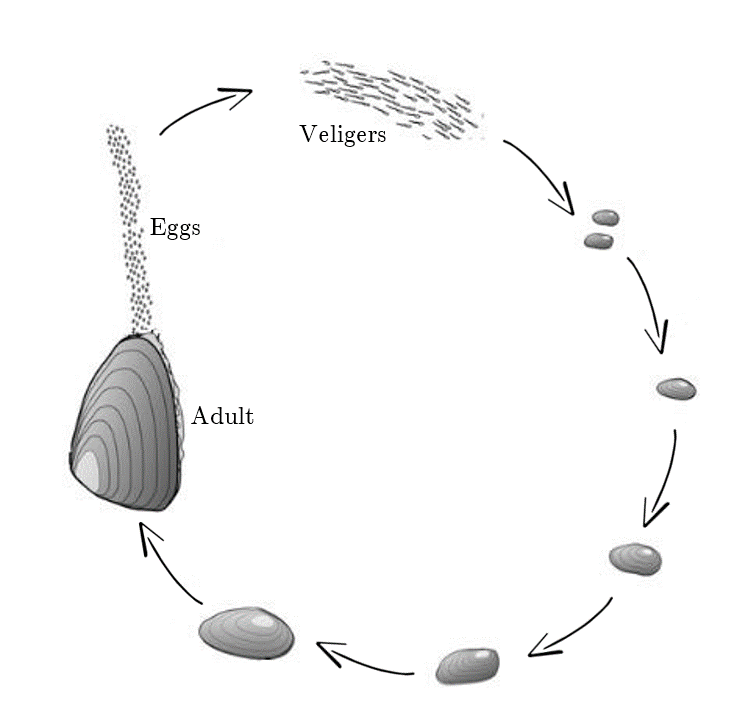
\includegraphics[scale = 0.6]{images/lifecycle}
	\caption{A diagram depicting the life cycle of dreissenid mussels.}
	\label{fig:lifecycle}
\end{figure}

Zebra mussels live between two and five years; they start as microscopic veligers but mature to thumbnail sized adults; they begin reproduction at two years of age, after which, females can release up to one million eggs per year \cite{NPS}. A diagram depicting the life cycle of dreissenid mussels is shown in Figure \ref{fig:lifecycle}. Dreissenid mussel veligers free-swim in the water; often, they travel to uninfested waters on boats or through other aquatic recreational activities, however, sometimes they are moved by nature and travel downstream to uninfested waters. Adult dreissenids attach and colonize hard surfaces in the water, this process of accumulation of adult zebra mussels on rocks, native mussels, docks, boats, or other hard surfaces is referred to as ``biofouling,'' and objects that are in the water for long periods of time become difficult and costly to clean.

Once a water body is colonized by adult dreissenid mussels, water supply and delivery facilities, water recreation sites, and other water dependent economies in that body of water become much more expensive to maintain and operate \cite{BOR}. For example, after dreissenid mussels were detected in Montana's Tiber Reservoir in 2016, with suspected detections in Canyon Ferry Reservoir as well, the state of Montana highlighted the economic impacts that a full dreissenid mussel colonization could have on the state; in January 2019, the Montana Department of Natural Resources and Conservation published a report titled \textit{Enumeration of Potential Economic Costs of Dreissenid Mussels Infestation in Montana}. The report states that if dreissenid mussels were to infest every lake and river in Montana, it could cost the state more than 230 million dollars annually in mitigation costs, as well as lost revenue \cite{MT}. 

Dreissenid infestations result not only in economic impacts, but in environmental ones as well. Dreissenid mussels are filter feeders and siphon plankton from the water, which can lead to changes the water body ecosystem by increasing water clarity; a single adult dreissenid can filter about a liter of water per day, which reduces the availability of algae for native mussels and bottom feeding fish \cite{BOR}. Additionally, ``biofouling'' can prevent native mussels from moving, feeding, reproducing, or regulating the water system. Several actions, such as the 2017 initiative, \textit{Safeguarding the West from Invasive Species}, by the Department of the Interior, have been taken to protect water bodies in the western United States from the economic and ecological threats posed by the invasive dreissenid mussels. Early detection of dreissenid mussels can reduce the economic and ecological repercussions of dreissenid infestations, however there are issues with the available early detection methods. 

The established standard for early detection of dreissenids in the western United States is plankton tow sampling for mussel veligers. Using a fine mesh net, water and debris are collected at multiple sampling sites within each water body; the debris from each net collected at the same sampling site on the same day is aggregated and examined, using cross-polarized light microscopy, for the free-swimming veligers. Following the microscopic examination, positive species identification is confirmed using polymerase chain reaction (PCR) chemistry. This early detection method requires a breeding population, so is limited to the weeks immediately following a spawning event \cite{Nichols}; spawning begins at water temperatures above 10$^\circ$C for quagga mussels and above 12$^\circ$C for zebra mussels \cite{McMahon, Mills}. This suggests that veliger availability in northern latitude water bodies is typically limited to warmer months \cite{Sepulveda:eDNA}.

An alternative method, growing in popularity, for detection of rare, endangered, or invasive species, is environmental DNA (eDNA) surveys \cite{Schmelzle}. Environmental DNA methods can detect DNA diffused by the target species in water sampled from a water body. Multiple water samples are collected from each sampling site within a lake, the samples are then analyzed using one of several different types of PCR chemistry. Sepulveda, Amberg, and Hanson (2019) suggest the use of eDNA surveys may widen the seasonal sampling window of plankton tow methods, since eDNA does not rely on a breeding population. Environmental DNA surveys are more time and cost effective than traditional sampling methods for species of low abundance \cite{Rees}. However, a positive eDNA result does not necessarily indicate that the target species is present or alive at the site; positive eDNA results can be obtained from ``a failed introduction, from external sources, or from field contamination, rather than fresh DNA from mussel colonization'' \cite{Sepulveda:eDNA}. One criticism of the detection of dreissenid mussels using eDNA is there is a possibility of obtaining false-positive results; since control efforts for invasive species are costly, there is some hesitation in using eDNA surveys as the sole decision-making tool for the management of dreissenid mussels. When the two early detection methods result in conflicting answers, decision making can be even more complicated, since a positive eDNA result suggests only that the DNA of the target species is present, regardless of whether the species is alive or even present at all, but when veligers are detected, positive eDNA results indicate a potential colonization, which is useful to managers \cite{Holser:body}. 

Occupancy models allow the occurrence of a species to be accurately estimated, even when the species is imperfectly detected. For both the plankton tow and eDNA surveys, there is a non-zero probability of a false negative result. Since plankton tow survey methods are restricted to capturing only mussel veligers, dreissenid mussels can be present in the lake and not be captured in the plankton tow nets at one or more of the sampling sites, either because the veligers are missed with the nets or because there are no free-swimming veligers available in the water; even if the veligers are captured in the net, there is a possibility that they are not detected using cross-polarized light microscopy. Similarly for eDNA methods, dreissenid mussels could be present in the lake, but their DNA could be missed in one or more of the samples from each of the sampling sites; even if dreissenid mussel DNA is present in the sample, it could be missed in the PCR replicate. Replication in the survey design can help researchers learn about the detection probabilities for each of the early detection methods. 

Land managers are often interested in the probability of occupancy in a given lake, whereas researchers are typically interested in detection probabilities. Furthermore, the researchers are also interested in recommendations on the number of samples necessary to ensure a high probability of at least one detection using digital droplet PCR (ddPCR) when dreissenid mussel eDNA is present at the site. The remainder of this exploration proceeds as follows: Section 2 briefly describes the data collection process and provides summary and visualization of the raw data; Section 3 contains a brief description of Bayesian statistical methods, a discussion of occupancy models and multi-scale occupancy models, and a few implementation methods for fitting the previously described models in \texttt{R}; Section 4 describes the analysis and the various models fit to the eDNA data; Section 5 covers the results from the models and their ecological implications; and finally, Section 6 briefly describes future work to be done on the project.

\section{Data}



The eDNA data were collected during the spring, summer, and fall of 2019 as part of a study on the detection of dreissenid mussels and Asian clams in northeastern lakes using environmental DNA. There were six lakes surveyed across Maine, New Hampshire, New York, and Vermont; each lake was sampled for dreissenid mussels, Asian clams, or both. The data available are from three of the lakes sampled for dreissenid mussels. There are multiple sites within each lake, from each, five one-liter water samples were collected. Most sites were visited on more than one day throughout the course of the study. Each of the samples were analyzed using a DNA amplification technique, known as digital droplet PCR (ddPCR), on a Biorad Digital Droplet PCR system using dreissenid mussel assays. This PCR technique divides the sample aliquot into micro droplets to be separately analyzed. A field blank of clean lab water accompanied the set of five samples from each site on a given day to ensure no cross contamination in the lab; these samples were removed from the data set. 

The lakes are coded ``BOM,'' ``LG,'' and ``MG,'' and these names will be used throughout. There are three sites in lake BOM (BOM1, BOM2, BOM3), each of which was sampled five times on three different days (May 28, July 8, and October 21), for a total of 15 samples per site and 45 total samples from lake BOM. There are five sites in lake LG; the first three sites (LG1, LG2, LG3) were sampled five times on both May 28 and July 8, and the final two sites (LG4, LG5) were each sampled five times on September 25, for a total of 40 samples from lake LG. There were originally five sites in lake MG, but one (MG2) was inaccessible on the study day, so there are data for four sites in lake MG (MG1, MG3, MG4, MG5), each of which was sampled five times on August 23, for a total of 20 samples from lake MG. In all, there are twelve sites and 105 samples. Each sample was filtered, and a portion of each of the filtered samples was divided into thousands of droplets for ddPCR analysis. Figure \ref{fig:eDNA_diagram} illustrates the hierarchical structure of the eDNA data within a lake. Ten sample rows of the data set are displayed in Table \ref{tab:eDNA_data}, where ``Positive Droplets'' is the number of droplets where dreissenid mussel DNA was amplified and ``Concentration'' is the copies of target DNA per microliter of extraction (copies/$\mu$L). Water temperatures ($^\circ$C) were also recorded at each sampling site on each study day, with the exception of temperatures at sites in lake BOM on October 21. 

\begin{figure}[]
	\centering
	
\includegraphics[scale = 0.7]{images/eDNA}
	\caption{A diagram displaying the hierarchical structure of the eDNA data.}
	\label{fig:eDNA_diagram}
\end{figure}

\begin{knitrout}
\definecolor{shadecolor}{rgb}{0.969, 0.969, 0.969}\color{fgcolor}\begin{table}[!h]

\caption{\label{tab:eDNA_table}\label{tab:eDNA_data}
             10 sample rows of the eDNA data.}
\centering
\resizebox{\linewidth}{!}{
\begin{tabular}[t]{ccccccc}
\toprule
Lake & Site & Sample & Date & Water Temperature & Concentration & Positive Droplets\\
\midrule
BOM & BOM1 & BOM1w0528195 & 5/28/2019 & 11.0 & 8.51 & 60\\
BOM & BOM1 & BOM1w0708194 & 7/8/2019 & 25.5 & 0.81 & 7\\
BOM & BOM2 & BOM2w1021191 & 10/21/2019 & NA & 1.14 & 8\\
BOM & BOM3 & BOM3w0528193 & 5/28/2019 & 6.0 & 178.72 & 1154\\
BOM & BOM3 & BOM3w0708193 & 7/8/2019 & 24.5 & 175.99 & 1388\\
BOM & BOM3 & BOM3w1021191 & 10/21/2019 & NA & 2.04 & 13\\
LG & LG1 & LG1w0528194 & 5/28/2019 & 12.0 & 0.00 & 0\\
LG & LG2 & LG2w0708194 & 7/8/2019 & 23.0 & 0.00 & 0\\
LG & LG2 & LG2w0708195 & 7/8/2019 & 23.0 & 0.00 & 0\\
MG & MG5 & MG5w082319D & 8/23/2019 & 18.3 & 0.00 & 0\\
\bottomrule
\end{tabular}}
\end{table}


\end{knitrout}



The number of positive droplets per sample range between 0 and 3331 for lake BOM, between 0 and 3 for lake LG, and between 0 and 2 for lake MG. Based on Figure \ref{fig:eDNA_droplets} it is clear that the samples taken on May 28 and July 8 from sites BOM2 and BOM3 tend to have the highest numbers of positive droplets, while the samples at the remaining sites across their respective sampling dates, and the samples taken on October 21 at sites BOM2 and BOM3 all have numbers positive droplets near 0. It is noted that samples with fewer than three positive droplets should be treated with caution, as they have potential to be false positives. This is immediately noticeable in lakes LG and MG, as all the values of positive droplets per sample are low for these two lakes. Of the 40 samples from lake LG, 38 of them resulted in no positive droplets, and the remaining two samples resulted in two or three positive droplets per sample. Similarly for lake MG, 16 of the 20 samples resulted in no positive droplets, and the remaining samples resulted in one or two positive droplets per sample. While larger numbers of positive droplets were observed in samples from lake BOM, there are still three samples which resulted in some, but fewer than three, positive droplets. 

\begin{figure}[]
\begin{knitrout}
\definecolor{shadecolor}{rgb}{0.969, 0.969, 0.969}\color{fgcolor}

{\centering 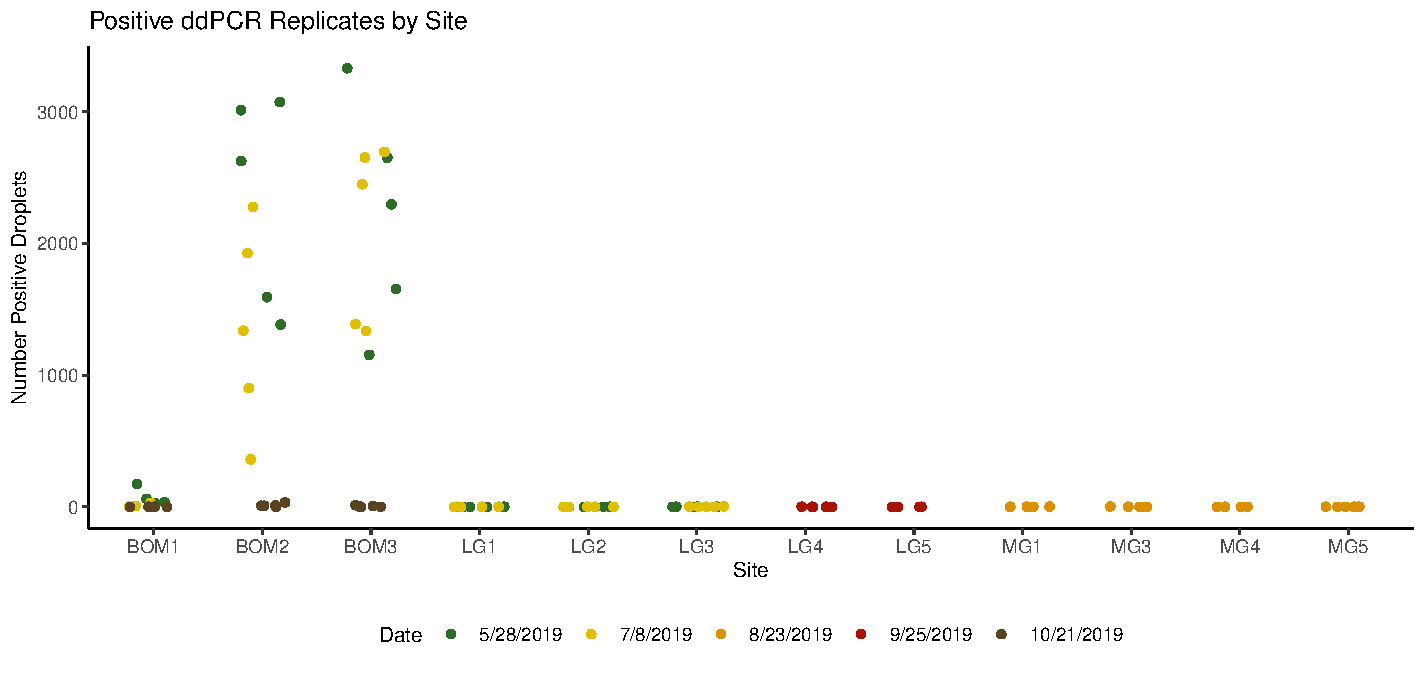
\includegraphics[width=\maxwidth]{figure/eDNA_visualization_droplets-1} 

}



\end{knitrout}
\caption{A plot of the positive droplets from each sample by site, colored by the date on which the sample was taken.}
\label{fig:eDNA_droplets}
\end{figure}

Somewhat related to the number of positive droplets in a sample, the concentrations in the study range between 0.00 and 733.80 copies/$\mu$L. Based on the top plot in Figure \ref{fig:eDNA_concentration}, it is clear that the sites with the highest concentrations occur in samples from sites BOM2 and BOM3, with average concentrations of 206 and 235 copies/$\mu$L in each of the respective sites. Sites LG1, LG2, LG4, LG5, and MG4 all have average concentrations of 0 copies /$\mu$L. The samples from the remaining sites tend to have low, but non-zero concentrations; the bottom plot in Figure \ref{fig:eDNA_concentration} displays the samples by site for non-zero concentrations below 10 copies/$\mu$L.  



\begin{figure}[]
\begin{knitrout}
\definecolor{shadecolor}{rgb}{0.969, 0.969, 0.969}\color{fgcolor}

{\centering 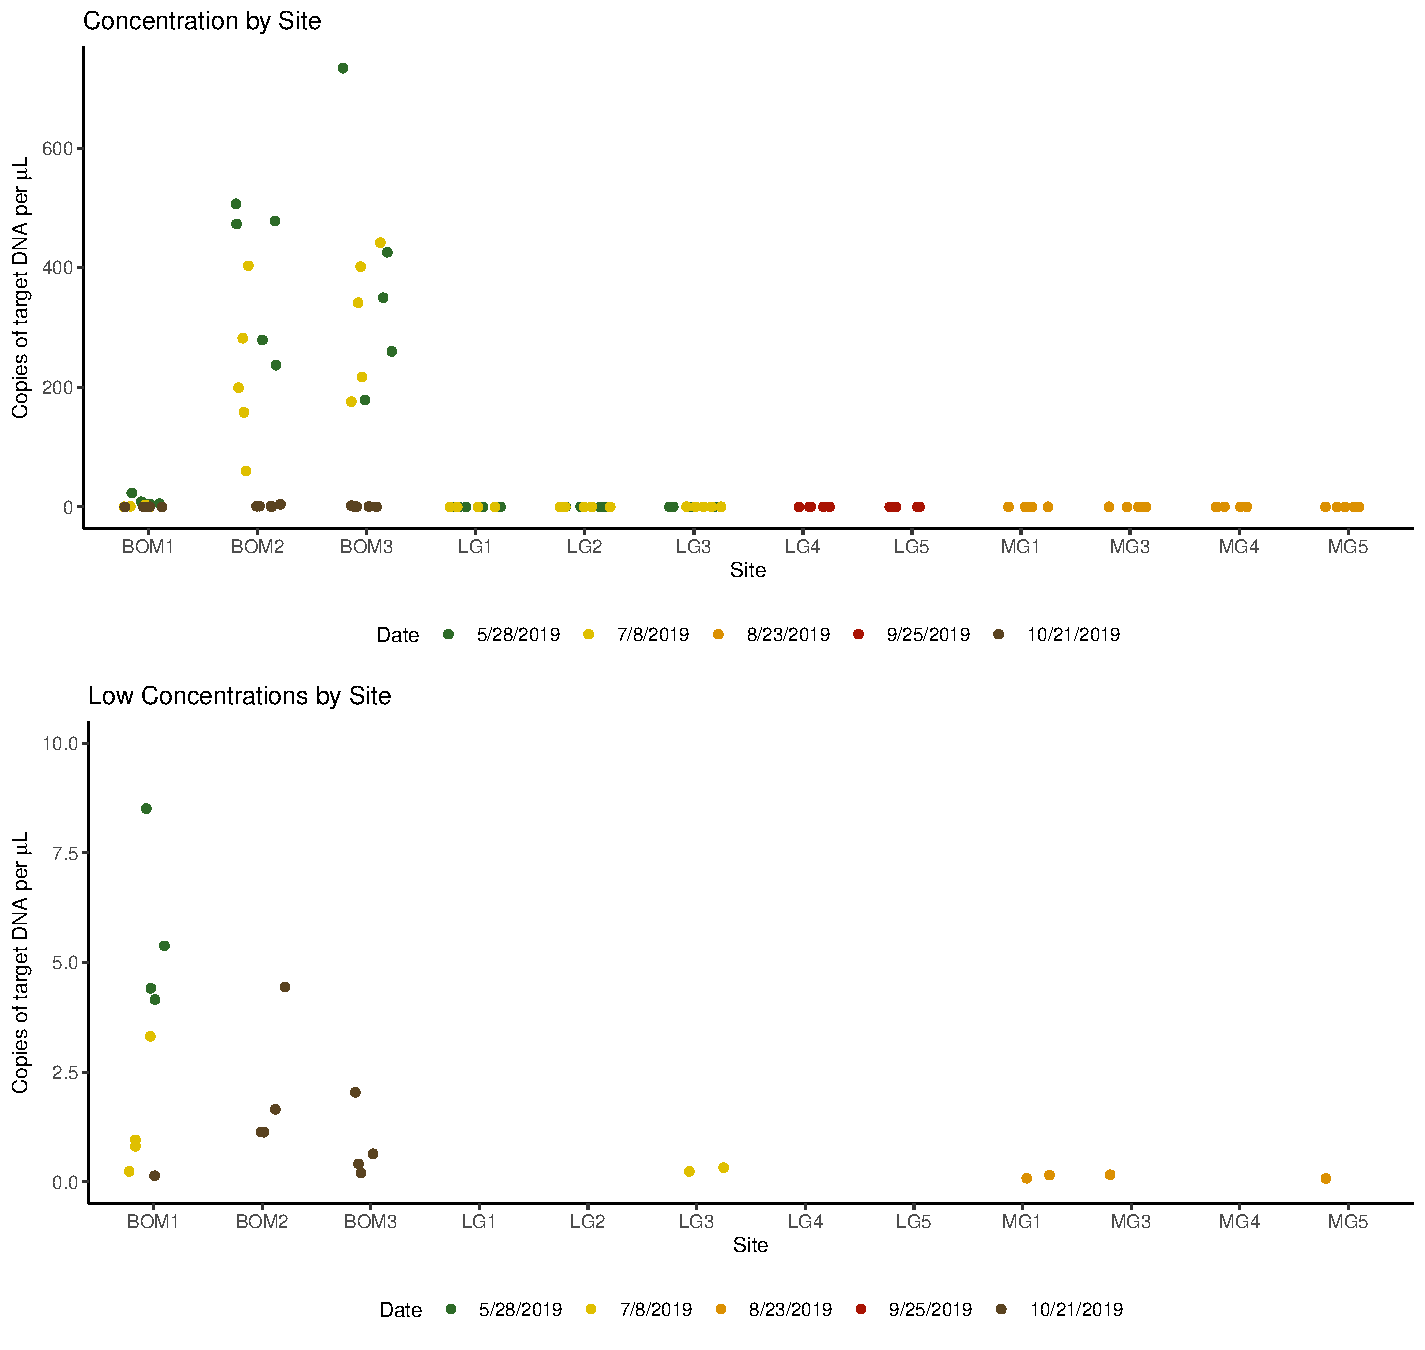
\includegraphics[width=\maxwidth]{figure/eDNA_visualization_concentration-1} 

}



\end{knitrout}
\caption{A plot displaying the number of copies of target DNA per $\mu$L per sample by site (top), and a plot displaying the number of copies of target DNA per $\mu$L for samples with low, but non-zero, concentrations (bottom).}
\label{fig:eDNA_concentration}
\end{figure}

\begin{figure}
\centering
\captionsetup[subfigure]{labelformat=empty}
\begin{subfigure}    
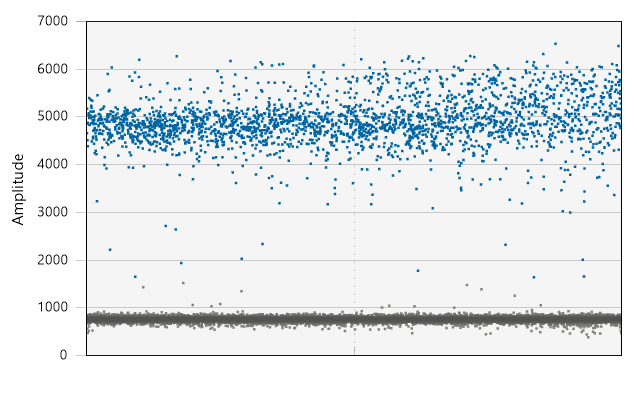
\includegraphics[scale = 0.6]{images/amplitude}   
\end{subfigure}
\begin{subfigure}
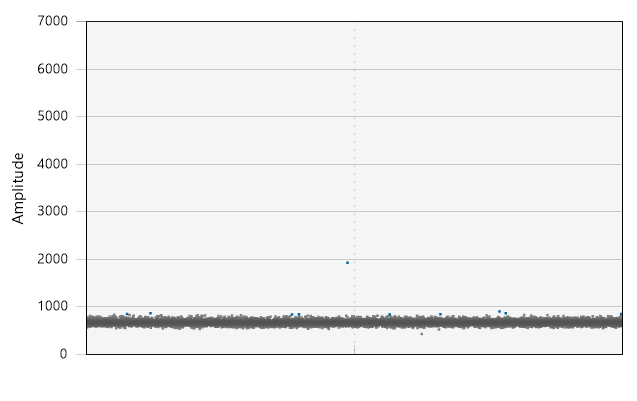
\includegraphics[scale = 0.6]{images/amplitude2}
\end{subfigure}
\caption{The droplet amplitudes for the second sample from site BOM3 on 7/8/2019 (top) and for the third sample from site LG5 on 9/25/19 (bottom).}
\label{fig:amplitudes}
\end{figure}

Since the number of positive droplets per sample is based on a subjective choice of amplitude cutoff to distinguish between positive and negative droplets, the number of positive droplets in a sample is arbitrary. The top plot in Figure \ref{fig:amplitudes} display the amplitudes of each droplet from the second sample from site BOM3 on 7/28/2019 and the bottom plot displays the amplitudes of each droplet from the third sample from site LG5 on 9/25/2019; the droplets with high amplitudes tend to suggest positive results. The band of blue points with amplitudes around 5000 in the top plot in Figure \ref{fig:amplitudes} are likely positive droplets, whereas the band of grey points with amplitudes less than 1000 in the same plot are likely negative droplets, however where to draw the line to distinguish between positive and negative droplets will change the number of positive droplets, perhaps dramatically in some samples. In the bottom plot in Figure \ref{fig:amplitudes}, the question becomes whether the droplet with an amplitude around 2000 should be considered positive or negative. To avoid basing the results on an arbitrary number of positive droplets, these data will be analyzed at the sample level. To limit the possibility of false positive detections for these analyses, to be considered a positive sample, the recommended threshold of three or more positive droplets will be used, therefore samples with three or more positive droplets will be considered positive samples. The top plot in Figure \ref{fig:eDNA_sample} displays the proportion of positive samples by site if all samples with positive droplets are treated as positive samples, and the bottom plot displays the proportion of positive samples by site using the above threshold to limit the positive sites to those with three or more positive droplets; the plots aid in understanding the changes in the proportion of positive samples from each site when the threshold is used. The application of the threshold changes the proportion of positive samples in six of the twelve sites. When the threshold is used, there are no positive samples observed in eight of the twelve sites. 



\begin{figure}[]
\begin{knitrout}
\definecolor{shadecolor}{rgb}{0.969, 0.969, 0.969}\color{fgcolor}

{\centering 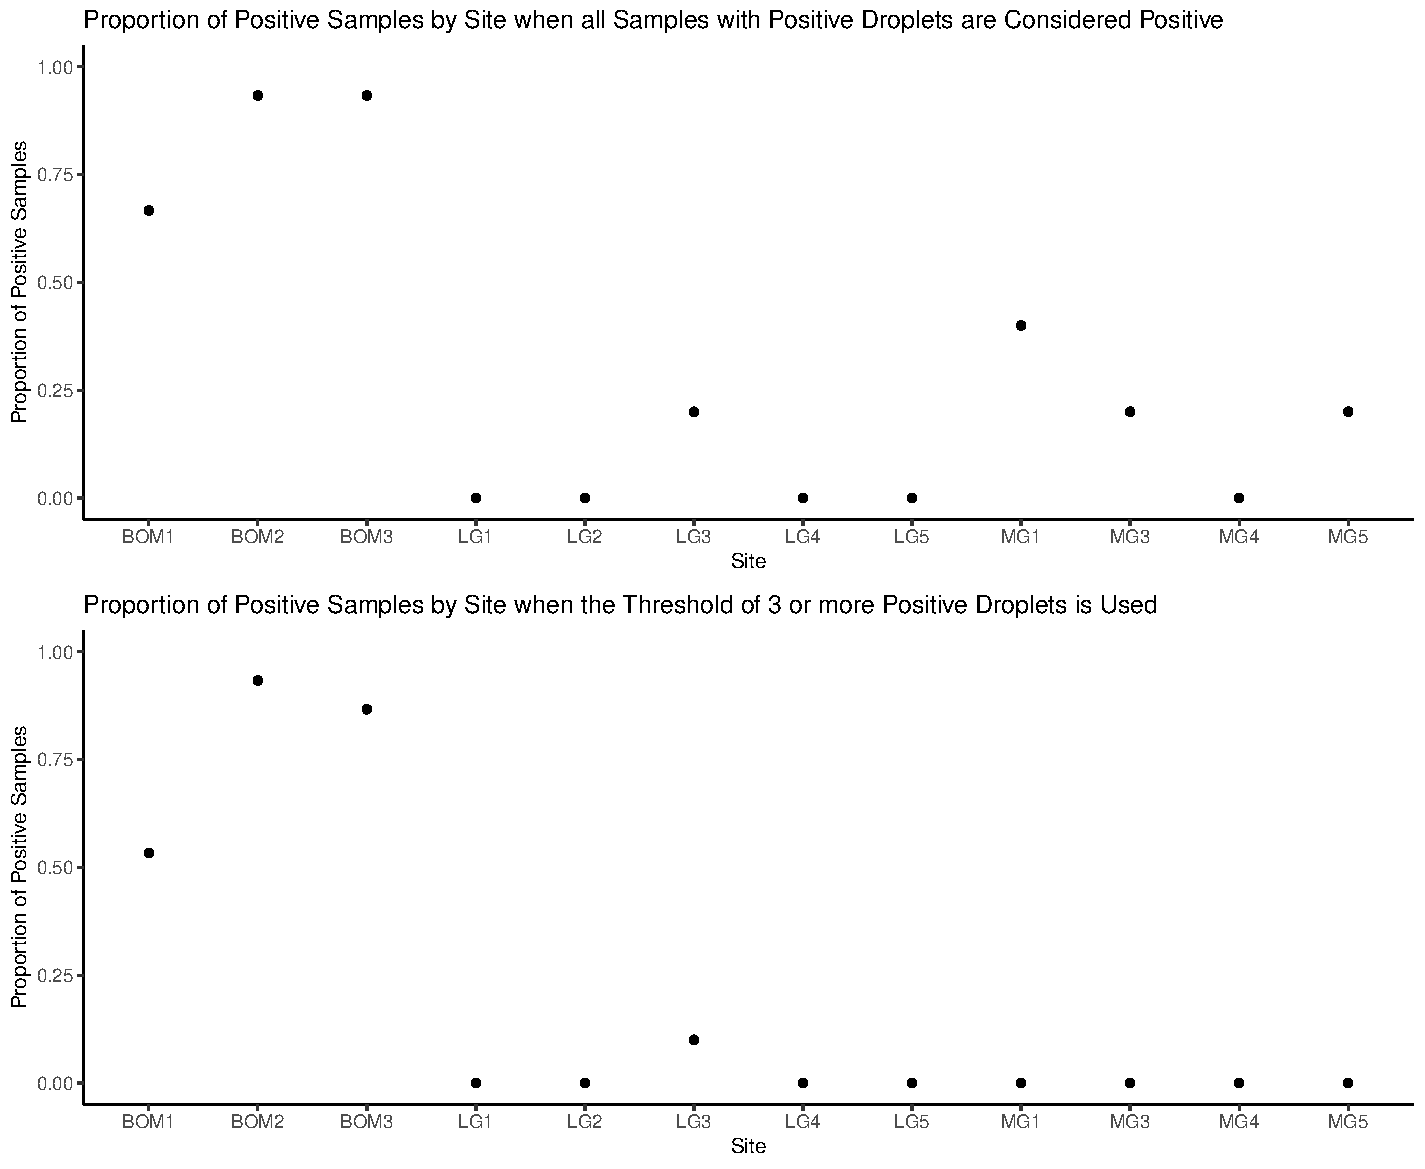
\includegraphics[width=\maxwidth]{figure/eDNA_visualization_sample-1} 

}



\end{knitrout}
\caption{A plot of the proportion of positive droplets by site if all samples with any positive droplets are treated as positive detections (top), and a plot of the proportion by site if samples with fewer than three positive droplets are treated as negative (bottom).}
\label{fig:eDNA_sample}
\end{figure}

Water temperature could impact the probability that dreissenid mussel eDNA is able to be detected using ddPCR. The water temperatures observed in lake BOM range from 6$^\circ$C to 25.5$^\circ$C, but temperatures were not recorded at any of the sites in lake BOM on October 21. The temperatures from a USGS gauge at a nearby lake, were positively adjusted by 2$^\circ$C to obtain an estimated temperature of 14$^\circ$C for all sites at lake BOM on October 21, 2019. The observed water temperatures in lake LG range from 12$^\circ$C to 23$^\circ$C, and from 17.2$^\circ$C to 18.9$^\circ$C in lake MG. Based on Figure \ref{fig:eDNA_temp}, it seems that the water temperatures on the same day are similar across sites within the same lake. For sites that were visited more than once, it is clear that water temperatures were cooler in the spring but warmed up in the summer. 

\begin{figure}[]
\begin{knitrout}
\definecolor{shadecolor}{rgb}{0.969, 0.969, 0.969}\color{fgcolor}

{\centering 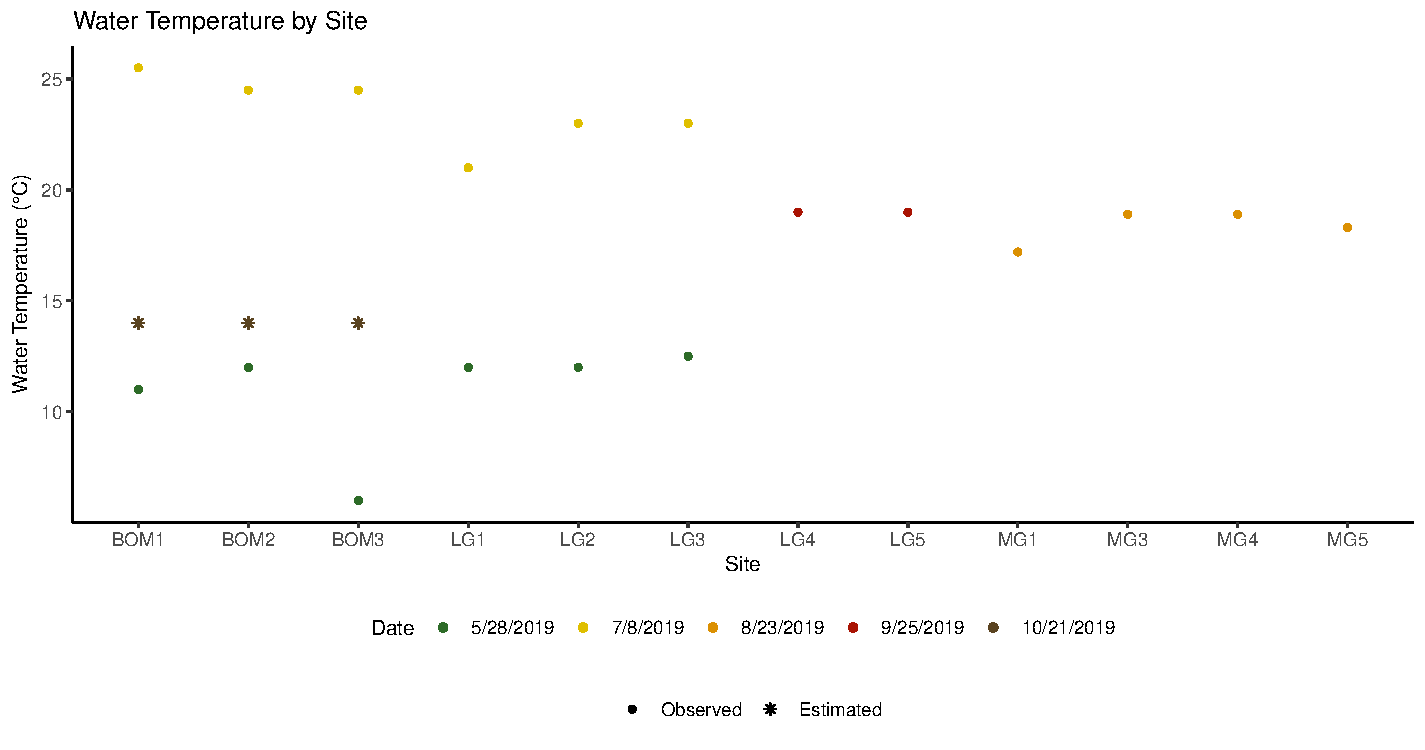
\includegraphics[width=\maxwidth]{figure/eDNA_visualization_temp-1} 

}



\end{knitrout}
\caption{A plot of the water temperatures by site, colored by the date on which the sample was taken. The estimated water temperatures are denoted with stars.}
\label{fig:eDNA_temp}
\end{figure}

\section{Methods}

\subsection{Bayesian Modeling Background}

In Bayesian statistics, inferences are based on the posterior distributions of the unknown parameters. The posterior distribution is a function of the likelihood of the observed data given a sampling model and some prior belief about the unknown parameters. Let $p(\bm{y}|\bm{\theta})$ denote the likelihood for some sampling model, and $p(\bm{\theta})$ denote the prior distribution on the unknown parameters $\bm{\theta}$. Then, using Bayes' rule, the posterior distribution, $p(\bm{\theta}|\bm{y})$, is: 

$$p(\bm{\theta}|\bm{y}) = \frac{p(\bm{y}|\bm{\theta})p(\bm{\theta})}{\int_\Theta p(\bm{y}|\bm{\theta})p(\bm{\theta})}$$

\noindent If the resulting posterior distribution is of the same distributional family as the prior distribution for the unknown parameter, then the prior is said to be conjugate for the sampling model. For example, if the observed data are $n$ independent binomial trails, with some unknown probability of success, $\theta$, and a beta prior distribution is used for $\theta$, it can be shown that the resulting posterior distribution is also a beta distribution. The complete model definition is: 

$$
\begin{aligned}
p(y_1, ..., y_n|\theta) &\sim binomial(n, \theta)\\
p(\theta) &\sim beta(\alpha, \beta)
\end{aligned}
$$

\noindent Using this, it can be shown that, 

$$p(\theta|y_1, ..., y_n) \sim beta \bigg( \sum_{i = 1}^n y_i + \alpha, n - \sum_{i = 1}^n y_i + \beta \bigg)$$

\noindent Therefore, since the prior distribution and the posterior distribution are of the same distributional family, then the beta prior is conjugate for the binomial sampling model.

However, the resulting posterior distribution is not always a named statistical distribution. In these situations, it is impossible to sample directly from the posterior distribution, but iterative sampling mechanisms can be used to approximate the unknown posterior distribution in order to make inferences. 

\subsubsection{Gibbs Sampler}

The most efficient iterative sampling technique available is the Gibbs sampler. In order to draw samples from an approximation of the joint posterior distribution using a Gibbs sampler, the full conditional posterior distribution of each of the unknown parameters must have a closed-form solution. The full conditional posterior distribution of a parameter is the distribution of that parameter, conditional on all other unknown parameters, the data, and the prior distributions. Once a full conditional posterior distribution is calculated for each unknown parameter, the iterative sampling can proceed in the following manner. 

\begin{mdframed}
\textit{Gibbs Sampler} \\
Let $\bm{\theta} = \{\theta_1, ..., \theta_p\}$ denote the vector of unknown parameters and $p(\theta_i|.)$ denote the full conditional distribution of $\theta_i$. The Gibbs Sampler generates the $s^{th}$ iteration as follows:
\begin{enumerate}
\item Sample $\theta_1^{(s)} \sim p(\theta_1|\theta_2^{(s-1)}, \theta_3^{(s-1)}, \dots, \theta_p^{(s-1)}, y_1, \dots, y_n)$. 
\item Sample $\theta_2^{(s)} \sim p(\theta_2|\theta_1^{(s)}, \theta_3^{(s-1)}, \dots, \theta_p^{(s-1)}, y_1, \dots, y_n)$.\\	
$\vdots$ \\[-14mm]
\item[$p$.] Sample $\theta_p^{(s)} \sim p(\theta_p|\theta_1^{(s)}, \theta_2^{(s)}, \dots, \theta_{p-1}^{(s)}, y_1, \dots , y_n)$. 
\end{enumerate}
\end{mdframed}

\noindent This process generates a dependent sequence of $\bm{\theta}$ vectors for each iteration, which together, converge to the joint posterior distribution, $p(\bm{\theta}|\bm{y})$. The Gibbs sampler is a basic Markov Chain Monte Carlo (MCMC) algorithm, where the current state only depends on the previous state, and additionally, the results should not depend on the starting values of $\bm{\theta}^{(0)}$.

One common use of a Gibbs sampler is for a normal sampling with unknown mean and variance. With this sampling model, a normal prior on the mean term and an inverse-gamma prior on the variance term enable the use of a Gibbs sampler to approximate the joint posterior distribution. However, in some cases, such as generalized linear models, semi-conjugate priors or closed-form solutions for the full conditional distributions are not available, and in those cases a Gibbs sampler cannot be used to sample from the joint posterior distribution of the unknown parameters. 

\subsubsection{Metropolis-Hastings Algorithm}

In cases that do not permit the use of a Gibbs sampler, a Metropolis-Hastings algorithm is often used to sample from the target distribution. Unlike a Gibbs sampler, a Metropolis-Hastings algorithm requires tuning, but proceeds in the following manner. 

\begin{mdframed}
\textit{Metropolis-Hastings Algorithm} \\
Let $\bm{\theta}^{(s)}$ be the current set of parameter estimates, $\bm{\theta}^*$ denote a new proposed set of parameters, and $J(\bm{\theta}^*|\bm{\theta}^{(s)})$ denote the proposal distribution, which is usually a random walk distribution. For example, $J(\bm{\theta}^*|\bm{\theta}^{(s)}) \sim MVN(\bm{\theta}^{(s)}, \gamma^2 \bm{I}_p)$ where $p$ is the number of unknown parameters, and $\gamma$ is thought of as the step size, or the average distance the proposed set of parameters falls from the current set. To complete an iteration: 
\begin{enumerate}
\item Sample $\bm{\theta}^*|\bm{\theta}^{(s)} \sim J(\bm{\theta}^*|\bm{\theta}^{(s)})$. 
\item Calculate the acceptance ratio $r = \frac{p(y|\bm{\theta}^*)p(\bm{\theta}^*)}{p(y|\bm{\theta}^{(s)})p(\bm{\theta}^{(s)})}$. 
\item Set $\bm{\theta}^{(s+1)}$:
\begin{itemize}
\item[-] If $r \geq 1$ then the proposed set, $\bm{\theta}^*$, is more attractive than the current set, $\bm{\theta}^{(s)}$, so $\bm{\theta}^{(s+1)} =   \bm{\theta}^*$. 
\item[-] If $r < 1$ then the proposed set, $\bm{\theta}^*$, is less attractive than the current set, $\bm{\theta}^{(s)}$, however the relative frequency of samples of $\bm{\theta}^*$ to $\bm{\theta}^{(s)}$ should be $r$, so with probability $r$, $\bm{\theta}^{(s+1)} = \bm{\theta}^*$.
\end{itemize}
\end{enumerate}
\end{mdframed}
  
\noindent The Metropolis algorithm is a generalization of the Metropolis-Hastings algorithm in which the proposal distribution is symmetric, meaning that $J(\bm{\theta}^*|\bm{\theta}^{(s)}) = J(\bm{\theta}^{(s)}|\bm{\theta}^*)$. The step size portion of the algorithm requires tuning and trace plots or other convergence tools should be used to ensure that the algorithm has efficiently explored the entire parameter space and converged to the true joint posterior distribution. 

\subsubsection{Bayesian Hierarchical Modeling}

Oftentimes data is collected in a hierarchical structure, that is data with a multilevel structure, such as students within classes, or sampling sites within a larger area of interest. For example, with two levels, the responses are independent observations from group $j$ and follow some distribution with unknown parameter $\theta_j$, meaning that $y_{1, j}, \dots, y_{n_j, j}|\theta_j \sim p(y|\theta_j)$; but the unknown parameters in each group are related to each other, such that they are independent samples from some distribution with parameter $\phi$, such that $\theta_1, \dots, \theta_m|\phi \sim p(\theta|\phi)$. With this representation, $p(y|\theta)$ is the variability among measurements within a group, and $p(\theta|\phi)$ is the sampling variability across groups. In order to completely specify the model, a prior distribution, $\phi \sim p(\psi)$, is needed for $\phi$. These models can be adapted to include covariates at each level, or to describe a more complicated structure with more levels. 

\subsection{Occupancy Models}

In ecological studies, there are several different state variables which may be of interest: abundance, vital rates, and occupancy are a few examples. Both mark-recapture and occupancy studies can be used to learn about the previously mentioned state variables, but there are advantages and limitations with each study type. In general, mark-recapture surveys are studies where individuals are capture or observed, given a unique mark, their identities recorded, and finally released; on subsequent occasions, both marked and unmarked individuals are captured, their identities recorded, unmarked individuals are marked, and they are all released. From this, capture histories, or encounter histories (typically a series of 0's and 1's) are recorded for each individual that is captured over the course of the study. There are several variations of mark-recapture studies, in which apparent survival, abundance, or both can be estimated depending on the study design. However, mark-recapture methods cannot be used when individuals of a species cannot be marked or uniquely identified. In this scenario, occupancy of a particular species can be recorded at each occasion. Occupancy methods are useful when studying a species over a large spatial scale for many years, particularly when the sampling sites are large relative to the species of interest. Though there is a loss in information about individuals of a species when occupancy studies are used, sometimes researchers are interested in the range of a species or the spread of invasion and therefore occupancy is the state variable of interest, and occupancy studies are most appropriate. Occupancy surveys are often used to track the mitigation efforts or spread of invasive species, but are plagued with imperfect detection probabilities. 

Occupancy models are a way to move past logistic regression for occupancy data in order to account for imperfect detection of the target species. However, multiple samples per site must be taken in order to learn about detection probabilities. For example, suppose five samples are taken from a site and two return a positive result, indicating that the species is present at the site, but the species was missed in three of the five samples, which provides information about the detectability of the species. There are several different types of occupancy models, but the traditional model is defined as follows. At the site level, $Z_i$ is defined as the presence ($Z_i = 1$) or absence ($Z_i = 0$) of the target species at the $i^{th}$ site ($i = 1, \dots, M$). Then, $Z_i \sim Bernoulli(\psi_i)$, where $\psi_i$ denotes the probability that the target species occupies the $i^{th}$ site. At the sample level, $Y_{ij}$ is defined as whether the target species is detected or not in the $j^{th}$ replicate at the $i^{th}$ site ($j = 1, \dots, J_{i}$). It follows that, $Y_{ij}|z_{ij} \sim Bernoulli(z_{i}p_{ij})$, where $z_i$ is the latent occupancy state for the $i^{th}$ site and $p_{ij}$ denotes the probability that the target species is detected on the $j^{th}$ survey, given the species occupies site $i$. The probability of detecting the target species at least one time given the species occupies the $i^{th}$ site can be calculated in the following manner: $p_i^* = 1 - \prod_{j = 1}^{J_i}(1 - p_{ij})$. Figure \ref{fig:ssocc} illustrates the structure of a traditional occupancy study, where each sample results in a binary response. 

\begin{figure}[]
	\centering
	
\includegraphics[scale = 0.7]{images/ssocc}
	\caption{A diagram displaying the structure of a traditional occupancy study.}
	\label{fig:ssocc}
\end{figure}

One assumption of occupancy models is that there is no unmodeled heterogeneity in the occupancy probabilities, or the detection probabilities, therefore covariates can be included at the site and sample levels. At the site level, $\bm{x}_i$ are the site specific covariates and $\bm{\beta}$ is the corresponding vector of regression parameters for $\psi_i$. At the sample level, $\bm{w}_{ij}$ are the sample specific covariates and $\bm{\alpha}$ is the corresponding vector of regression parameters for $p_{ij}$. It is also assumed that the sites are closed to changes in occupancy, so a site that is occupied at the beginning of the study should remain occupied throughout; if an occupancy study takes place over many years, there are models to account for the potential changes in occupancy status at the sites. Another assumption of these models is that the species is not misidentified, however, there are models that can account for false negative and false positive detections. The final assumption of these models is that the detection of the species is independent across sites. Violations of these assumptions can result in biased estimates of the occupancy and detection probabilities. 

\subsubsection{Multi-scale Occupancy Models}

For more illusive species, the samples from each site are often split into sub-samples, or replicates, and analyzed on a smaller scale. This introduces a hierarchical structure in the data creating dependencies which need to be accounted for \cite{MacKenzie}. One modeling approach to these types of data is the hierarchical latent state multi-scale occupancy model defined by Dorazio and Erickson which accounts for false negatives at the site, sample, and replicate levels \cite{Dorazio_Erickson}. The model is defined similarly to the traditional occupancy model described above, with an additional replicate level, the notation is as follows. At the site level, $Z_i$ is defined as the presence ($Z_i = 1$) or absence ($Z_i = 0$) of the target species at the $i^{th}$ site ($i = 1, \dots, M$). Then, $Z_i \sim Bernoulli(\psi_i)$, where $\psi_i$ denotes the probability that the target species occupies the $i^{th}$ site. At the sample level, $A_{ij}$ is defined as the presence or absence of the target species in the $j^{th}$ sample from the $i^{th}$ site ($j = 1, \dots, J_i$). Then, $A_{ij}|z_i \sim Bernoulli(z_i\theta_{ij})$, where $z_i$ is the latent occupancy state for the $i^{th}$ site, and $\theta_{ij}$ is the conditional probability that the target species is present in the $j^{th}$ sample from the $i^{th}$ site, given the target species is present at the site. At the replicate level, $Y_{ijk}$ is defined as whether the target species is detected or not in the $k^{th}$ replicate of the $j^{th}$ sample collected at the $i^{th}$ site ($k = 1, \dots, K_{ij}$). It follows that, $Y_{ijk}|a_{ij} \sim Bernoulli(a_{ij}p_{ijk})$, where $a_{ij}$ is the latent occupancy state for sample $j$ from site $i$, and $p_{ijk}$ is the conditional the probability that the target species is detected in the $k^{th}$ replicate of the $j^{th}$ sample collected at the $i^{th}$ site, given the target species is present in that sample. If $p_{ijk}$ does not differ among the replicates and the replicates are statistically independent, the replicate level can be simplified in the following manner: $Y_{ij}|a_{ij} \sim binomial(K_{ij}, a_{ij}p_{ij})$, where $Y_{ij} = \sum_{k = 1}^{K_{ij}}Y_{ijk}$, and $p_{ij}$ is the conditional probability of detection in each replicate of the $j^{th}$ sample collected at the $i^{th}$ location, given that the target species is present in that sample. Similarly to above, an assumption of these models is that there is no unmodeled heterogeneity in the detection and occupancy probabilities, so covariates can be included in each level of the model to account for differences between individual sites, samples, or replicates; the notation for the covariates and corresponding regression parameters for the multi-scale occupancy model are as follows. At the site level, $\bm{x}_i$ are the site specific covariates and $\bm{\beta}$ is the corresponding vector of regression parameters for $\psi_i$. At the sample level, $\bm{w}_{ij}$ are the sample specific covariates and $\bm{\alpha}$ is the corresponding vector of regression parameters for $\theta_{ij}$. At the replication level, where there are no replicate level covariates, $\bm{v}_{ij}$ are the sample specific covariates and $\bm{\delta}$ is the corresponding vector of regression parameters for $p_{ij}$. Site specific covariates can be included for $\theta_{ij}$ and $p_{ij}$. The remaining assumptions from traditional occupancy models, described above, hold for multi-scale occupancy models as well.  

When summarized at the sample level, the data could be modeled in a traditional occupancy framework or a multi-scale occupancy framework. With the occupancy probability modeled at the sampling site level and detection probability modeled at the sample level, the data fit into a traditional occupancy model; however, with the occupancy probability modeled at the lake level, the availability modeled at the sampling site level, and the detection probability modeled at the sample level, the data fit into a multi-scale occupancy model. Finally, if analyzed at the droplet level the data could be analyzed with a multi-scale occupancy model where the occupancy probability is modeled at the sampling site level, availability modeled at the sample level, and the detection probability modeled at the droplet level. As previously mentioned, the data will be summarized at the sample level and analyzed in a traditional occupancy model framework. 

\subsection{Implementation}

There are several options for fitting occupancy models; the \texttt{R} package used for this analysis as well as some alternative methods for fitting occupancy models are described below. 

\subsubsection{\texttt{Rcppocc} Package for Fitting Occupancy Models}

The traditional occupancy model described above can be fit in a Bayesian framework with the \texttt{PGocc4()} function from the \texttt{R} package \textt{Rcppocc} \cite{Rcppocc}. This package relies on \texttt{Rcpp} and \texttt{RcppArmadillo}, so the models are computationally efficient. Additionally, the \texttt{PGocc4()} function introduces P\'{o}lya Gamma latent variables into the model to enable the use of a Gibbs sampler with the logit link function, while alternative options often use a Gibbs sampler with a probit link function, or a Metropolis-Hastings algorithm in conjunction with the logit link function. The use of a Gibbs sampler over a Metropolis-Hastings algorithm is generally preferred since the Gibbs sampler does not require tuning and is more computationally efficient. The interpretations of the estimated coefficients are not as straight-forward for the probit link function as they are when the logit link function is used, therefore this package provides the best of both worlds in terms of sampling algorithms and link functions for the regression parameters.  

\subsubsection{\texttt{msocc} Package for Fitting Multi-scale Occupancy Models}

The multi-scale occupancy model described above \cite{Dorazio_Erickson} can be easily fit in a Bayesian framework with the \texttt{msocc} package in \texttt{R} \cite{Stratton}. This package implements the P\'{o}lya Gamma data augmentation strategy described by Polson et. al (2013) to enable the use of a Gibbs sampler in conjunction with a logit link function. The model is specified in a familiar way to users of \texttt{R} at each level of the hierarchy in the model fitting function \texttt{msocc\_mod()}. To make the package more computationally efficient, there is an option to use the Beta-Binomial sampler when possible. Other functionalities of the package are the posterior summary tools (\texttt{posterior\_summary()}) and the function for generating credible interval plots (\texttt{cred\_plot()}) at all levels of the hierarchy. 

\subsubsection{Alternative Options}

There are several alternative options for fitting occupancy models. For example, the \texttt{eNDAoccupancy} \cite{Dorazio_Erickson} package fits the Bayesian multi-scale occupancy model defined above using a Metropolis-Hastings algorithm, which is less efficient and requires tuning. Occupancy models can also be written in \texttt{STAN} or \texttt{JAGS} and run in \texttt{R} using the packages \texttt{rstan} \cite{rstan} and \texttt{rjags} \cite{rjags} respectively, but again these methods are less computationally efficient than the methods described above. There are various frequentist methods for fitting occupancy models as well. A commonly used \texttt{R} package for fitting frequentist occupancy models is \texttt{unmarked} \cite{unmarked}. Ecologists often utilize Program MARK, or access its functionalities through the \textt{R} package \texttt{RMark} \cite{RMark} to fit occupancy models, and other various models popular in ecology.

\section{Analysis}

For these data, the occupancy probabilities can be estimated as constant across the sites, estimated by lake, or estimated individually for each site. Since the sites are across three different lakes, a constant occupancy probability across sites does not make sense, because different bodies of water have different water chemistry that could impact whether dreissenid mussel eDNA is present. However, estimating an individual occupancy probability for each site is likely more than necessary, because once a site is occupied with dreissenid mussels, it makes sense that the entire lake should be considered occupied, therefore occupancy probabilities will be estimated as constant for sites within the same lake. There are more options for covariates to impact the detection probabilities in each sample, conditional on site occupancy. It seems reasonable to assume that, conditional on site occupancy, the probability of detection depends on water temperature to allow for heterogeneity in detection probabilities across sites. The assumption of no unmodeled heterogeneity in the occupancy probabilities or the detection probabilities seems reasonable here, though it would be nice to include water chemistry variables at the site level that are thought to impact whether a dreissenid mussel population can flourish. The sites in the study are assumed to be independent; in this case, there are multiple sites within each lake, which would violate the independence assumption if not accounted for in the model. After lake is accounted for, from my understanding of site locations within a lake, it seems reasonable for the sites to be considered independent. The likelihood of false positive detections were limited by using the recommended threshold of three or more positive droplets to be considered a positive sample, however the one site in lake LG with one positive sample only contained three positive droplets. The sites are also assumed to be closed to changes in occupancy throughout the course of the study, there is limited knowledge about how long eDNA remains in the water or how it moves throughout the water, so there is potentially some violation of the closure assumption, however, if the eDNA moves in and out of the sites randomly throughout the course of the study, the $\psi$ parameter estimates will be unbiased. The model statements for the probability parameters are as follows :  

$$
\begin{aligned}
logit(\psi_i) &= \beta_0 + \beta_1I_{lake = LG, i} + \beta_2I_{lake = MG, i}\\
logit(p_{ij}) &= \alpha_0 + \alpha_1water.temp_{ij}
\end{aligned}
$$

\noindent where the $I_{lake = LG, i}$ is an indicator variable that is 1 when the $i^{th}$ site is in lake LG and 0 otherwise, $I_{lake = MG, i}$ is a similarly defined indicator variable, which is 1 when the $i^{th}$ site is in lake MG and 0 otherwise, and $water.temp_{ij}$ is the water temperature for the $j^{th}$ sample from the $i^{th}$ site. 

Prior distributions are needed for each vector of regression coefficients, $\bm\beta$ and $\bm\alpha$. The following prior distributions were used: 
$$
\begin{aligned}
\bm{\beta} &\sim MVN(\tilde 0, 100^2I)\\
\bm{\alpha} &\sim MVN(\tilde 0, 100^2I).
\end{aligned}
$$

\noindent The multivariate normal distribution centered at $\tilde 0$ places equal prior probability on each of the $\beta$ and $\alpha$ coefficients being positive or negative; a covariance matrix of $100^2 I$ places a relatively flat prior distribution on each of the $\beta$ and $\alpha$ coefficients.






































\section{Results}



\begin{table}[!h]
\caption{\label{tab:m5_beta}
             Summary table of the $\hat \beta$ coefficients for $logit(\hat \psi_i) = \hat \beta_0 + 
             \hat \beta_1I_{lake = LG, i} + \hat \beta_2I_{lake = MG, i}$.}
\small
\centering {
\begin{tabular}[t]{lrrr}
\toprule
  & \multicolumn{1}{c}{Mean} & \multicolumn{1}{c}{\begin{tabular}[c]{@{}c@{}}2.5\% \\ Quantile\end{tabular}} & \multicolumn{1}{c}{\begin{tabular}[c]{@{}c@{}}97.5\% \\ Quantile\end{tabular}}\\
\midrule
$\hat\beta_0$ & 40.77509 & 2.78929 & 121.46364 \\
$\hat\beta_1$ & -42.58740 & -123.55015 & -4.36077 \\
$\hat\beta_2$ & -107.34176 & -235.01267 & -21.15072 \\
\bottomrule
\end{tabular}}
\end{table}

Based on the $\beta$ estimates in Table \ref{tab:m5_beta} it appears that the log-odds of occupancy is different in each of the three lakes. Additionally, based on the $\alpha$ estimates in Table \ref{tab:m5_alpha}, for a 1$^\circ$C increase in water temperature, the estimated odds of detecting dreissenid mussel eDNA with ddPCR is between 0.95 and 1.25 times what it would have been previously, with 95\% probability. This suggests that water temperature might not impact sample level detection probabilities, but it will be retained in the model to control for differences that could arise in detection probabilities.  



\begin{table}[!h]
\caption{\label{tab:m5_alpha}
             Summary table of the $\hat \alpha$ coefficients for $logit(\hat p_{ij}) = \hat \alpha_0 +
             \hat \alpha_1water.temp_{ij}$.}
\small
\centering {
\begin{tabular}[t]{lrrr}
\toprule
  & \multicolumn{1}{c}{Mean} & \multicolumn{1}{c}{\begin{tabular}[c]{@{}c@{}}2.5\% \\ Quantile\end{tabular}} & \multicolumn{1}{c}{\begin{tabular}[c]{@{}c@{}}97.5\% \\ Quantile\end{tabular}}\\
\midrule
$\hat\alpha_0$ & 0.09886 & -0.93826 & 1.13725 \\
$\hat\alpha_1$ & 0.08632 & -0.04662 & 0.22648 \\
\bottomrule
\end{tabular}}
\end{table}

Perhaps more interesting than the $\alpha$ and $\beta$ estimates themselves, especially to land managers and researchers are the probability estimates derived from those estimated $\alpha$'s and $\beta$'s.

\subsection{Ecological Implications}

Based on the model, there is a 95\% chance that the probability dreissenid mussel eDNA is present in lake BOM is between 94.2\% and 100\% (posterior mean occupancy probability for lake BOM: 99.4\%). Additionally, there is a 95\% chance that the probability dreissenid mussel eDNA is present in lake MG is between 0\% and 1.7\% (posterior mean occupancy probability for lake MG: 0.2\%). However, there is much less certainty about the occupancy status of lake LG; there is a 95\% chance that the probability dreissenid mussel eDNA is present in lake LG is between 0.6\% and 61.5\% (posterior mean occupancy probability for lake LG: 20.3\%). Figure \ref{m5_cred_psi} displays visually the 95\% credible intervals and posterior means for each of the $\hat\psi_i$. These results suggest that we are fairly confident that lake BOM contains dreissenid mussel eDNA, lake MG does not, but we are unsure about the whether lake LG contains dreissenid mussel eDNA. 

\begin{figure}
\begin{knitrout}
\definecolor{shadecolor}{rgb}{0.969, 0.969, 0.969}\color{fgcolor}
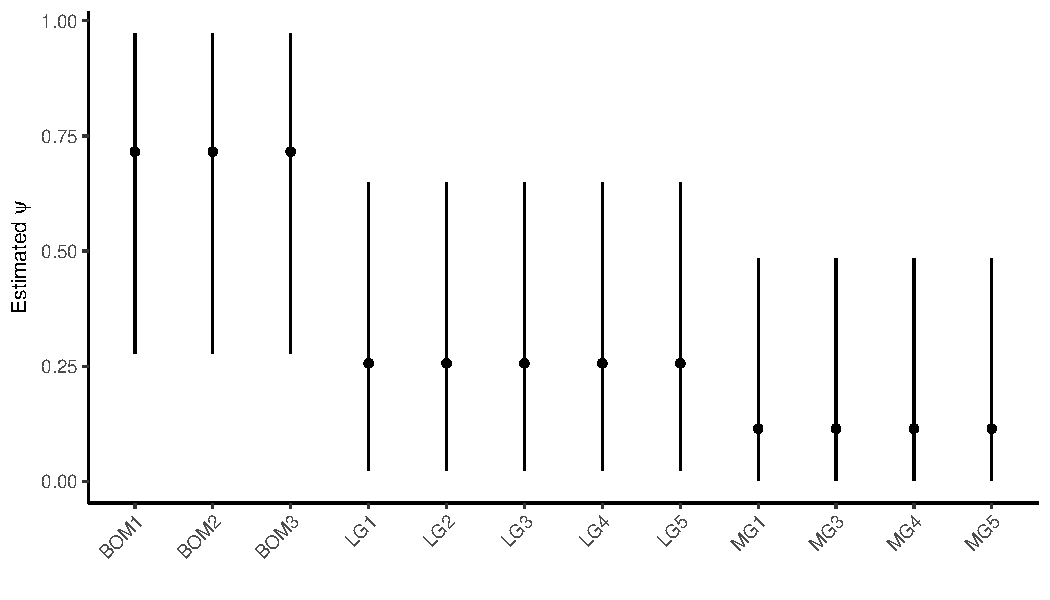
\includegraphics[width=\maxwidth]{figure/m5_psi-1} 

\end{knitrout}
\caption{Plot of the 95\% credible intervals for each of the $\hat\psi_i$, the posterior mean is plotted with a point.}
\label{fig:m5_cred_psi}
\end{figure}

Of further interest to researchers are the detection probabilities for each sample. In this model, detection probabilities were allowed to vary by water temperature, so each of the five samples on the same day from each site should have the same detection probability estimates because multiple water temperatures were not recorded within the same site on the same day. A plot of the 95\% credible intervals and posterior means for each uniquely estimated detection probability is plotted by site and date in Figure \ref{fig:m5_cred_p}; based on the figure, it appears that the detection probabilities, conditional on site occupancy, vary slightly. Table \ref{tab:m5_p_table} displays the numerical summaries of the estimated detection probabilities, conditional on site occupancy. 

\begin{figure}
\begin{knitrout}
\definecolor{shadecolor}{rgb}{0.969, 0.969, 0.969}\color{fgcolor}
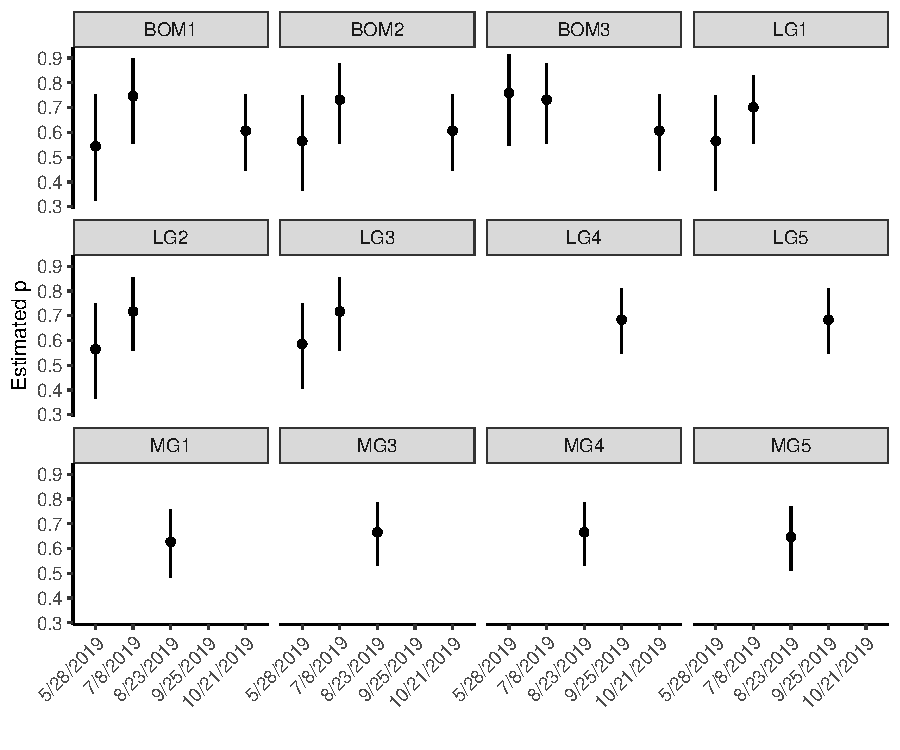
\includegraphics[width=\maxwidth]{figure/m5_p-1} 

\end{knitrout}
\caption{Plot of the 95\% credible intervals for each of the uniquely estimated $p_{ij}$, the posterior mean is plotted with a point.}
\label{fig:m5_cred_p}
\end{figure}


\begin{table}[!h]
\caption{\label{tab:m5_p_table}
             Summary table of the estimated detection probabilities for each site and date combination; the water temperatures are provided and the temperatures that were estimated in lake BOM on 10/20/2019 are denoted with $^\bm{*}$.}
\small
\centering {
\begin{tabular}[t]{lrrrrr}
\toprule
\multicolumn{1}{c}{Site} & \multicolumn{1}{c}{Date} & \multicolumn{1}{c}{\begin{tabular}[c]{@{}c@{}}Water \\ Temp. ($^\circ$C) &\end{tabular}} & \multicolumn{1}{c}{Mean} & \multicolumn{1}{c}{\begin{tabular}[c]{@{}c@{}}2.5\% \\ Quantile\end{tabular}} & \multicolumn{1}{c}{\begin{tabular}[c]{@{}c@{}}97.5\% \\ Quantile\end{tabular}}\\
\midrule
BOM1 & 5/28/2019 & 11 & 0.54382 & 0.32368 & 0.75231 \\
BOM1 & 7/8/2019 & 22.5 & 0.74579 & 0.55351 & 0.89687 \\
BOM1 & 10/21/2019 & 14$^\bm{*}$ & 0.60643 & 0.44682 & 0.75239 \\
BOM2 & 5/28/2019 & 12 & 0.56473 & 0.36574 & 0.75031 \\
BOM2 & 7/8/2019 & 24.5 & 0.73189 & 0.55687 & 0.87688 \\
BOM2 & 10/21/2019 & 14$^\bm{*}$ & 0.60643 & 0.44682 & 0.75239 \\
BOM3 & 5/28/2019 & 6 & 0.75864 & 0.54867 & 0.91416 \\
BOM3 & 7/8/2019 & 24.5 & 0.73189 & 0.55687 & 0.87688 \\
BOM3 & 10/21/2019 & 14$^\bm{*}$ & 0.60643 & 0.44682 & 0.75239 \\
LG1 & 5/28/2019 & 12 & 0.56473 & 0.36574 & 0.75031 \\
LG1 & 7/8/2019 & 21 & 0.70083 & 0.55391 & 0.83139 \\
LG2 & 5/28/2019 & 12 & 0.56473 & 0.36574 & 0.75031 \\
LG2 & 7/8/2019 & 23 & 0.71690 & 0.55778 & 0.85484 \\
LG3 & 5/28/2019 & 12.5 & 0.58567 & 0.40791 & 0.75002 \\
LG3 & 7/8/2019 & 23 & 0.71690 & 0.55778 & 0.85484 \\
LG4 & 9/25/2019 & 19 & 0.68371 & 0.54598 & 0.80815 \\
LG5 & 9/25/2019 & 19 & 0.68371 & 0.54598 & 0.80815 \\
MG1 & 8/23/2019 & 17.2 & 0.62680 & 0.48230 & 0.75898 \\
MG3 & 8/23/2019 & 18.9 & 0.66559 & 0.53281 & 0.78707 \\
MG4 & 8/23/2019 & 18.9 & 0.66559 & 0.53281 & 0.78707 \\
MG5 & 8/23/2019 & 18.3 & 0.64658 & 0.51140 & 0.77118 \\
\bottomrule
\end{tabular}}
\end{table}

\subsection{Sampling Recommendations}

Of further interest to the researchers is sampling recommendations, such as the recommended number of samples to take to ensure a high probability of at least detection at a site, if the site is occupied. A table of probabilities of detecting dreissenid mussel eDNA at least one time in the $J_i$ samples from each of the twelve sites, given that there is dreissenid mussel eDNA present at the $i^{th}$ site is provided in Table \ref{tab:m5_pstar_table}. Based on this model, the estimated probabilities of detecting dreissenid mussel eDNA in at least one sample from the $i^{th}$ site, given dreissenid mussel eDNA is present at the site, is high across all the sites, with a lower bound of 97\%. This suggests that the number of sampling scheme used for this study is sufficient. However, these detection probabilities are driven by the detections at lake BOM. Since the occupancy probabilities and detection probabilities are interwoven in their estimation, more samples at lake LG and MG could help researchers get a better idea about the detection probabilities at sites that are potentially occupied but have low abundance of dreissenid mussel eDNA. 
 


\begin{table}[!h]

\caption{\label{tab:m5_pstar_table}
             Summary table of the estimated probabilities of detecting dreissenid mussel eDNA at least one time in the $J_i$ samples, given there is dreissenid mussel eDNA present at the $i^{th}$ site.}
\small
\centering {
\begin{tabular}[t]{lcrr}
\toprule
\multicolumn{1}{c}{Site} & \multicolumn{1}{c}{\begin{tabular}[c]{@{}c@{}}Number of\\ Samples\end{tabular}} & \multicolumn{1}{c}{\begin{tabular}[c]{@{}c@{}}2.5\% \\ Quantile\end{tabular}} & \multicolumn{1}{c}{\begin{tabular}[c]{@{}c@{}}97.5\% \\ Quantile\end{tabular}}\\
\midrule
BOM1 & 15 & 1.000 & 1.000 \\
BOM2 & 15 & 1.000 & 1.000 \\
BOM3 & 15 & 1.000 & 1.000 \\
LG1 & 10 & 0.998 & 1.000 \\
LG2 & 10 & 0.998 & 1.000 \\ 
LG3 & 10 & 0.999 & 1.000 \\
LG4 & 5 & 0.981 & 1.000 \\
LG5 & 5 & 0.981 & 1.000 \\
MG1 & 5 & 0.963 & 0.999 \\
MG3 & 5 & 0.978 & 1.000 \\
MG4 & 5 & 0.978 & 1.000 \\
MG5 & 5 & 0.971 & 0.999 \\
\bottomrule
\end{tabular}}
\end{table}

As previously mentioned, it would also be of interest to collect other water chemistry variables thought to impact whether a dreissenid mussel population is able to establish, such as dissolved calcium and pH \cite{ZM_facts}; these covariates could be included in the modeling for the occupancy parameters, which would better inform why the sites differ in terms of occupancy. 

After the samples are collected and filtered, it would be beneficial to take multiple sub-samples from the filtered water. This would hopefully lead to an understanding of where some of the missed detections are coming from. There are multiple ways a negative sample can arise: there is no dreissenid mussel eDNA at the site; there is dreissenid mussel eDNA at the site but it is not captured in the sample; the dreissenid mussel eDNA is present at the site, is captured in the sample, but not be captured in the sub-sample that was analyzed with ddPCR; or there the dreissenid mussel eDNA is present at the sites, is captured in the sample, is captured in the sub-sample, but is not detected with ddPCR. If multiple sub-samples, or replicates, were taken from the same sample, more could be learned about where the missed detections are occurring in the process.

\section{Future Work}

Oftentimes in occupancy surveys, there is potential for another species to be misidentified as the species of interest in the study, this would lead to a false positive results. In eDNA surveys, false positives likely occur as a result of the PCR technique. With digital droplet PCR, there is a chance that optical interference could lead to false positive results. False positives have the potential to positively bias the detection probabilities, which in turn, can negatively bias the occupancy probabilities. In the near future, the plan is to model these data with an occupancy model that accounts for false positive detections. If a false positive occupancy model is used, the threshold of the number of droplets to be considered a positive sample can be excluded, and all samples with any number of positive droplets can be considered positive samples, since the model itself would allow for false positive detections. There are various different options for false positive occupancy models. One example is the model defined by Royle and Link (2006), in which there is symmetry in the likelihood which leads to solutions that are not unique. To account for this, the parameter space is restricted in the model such that the true positive detection probability is greater than the false positive detection probability. However, this restriction was criticized by McClintock et al. because if the the target species is not present and is falsely detected, then the conclusion would be that the species is present due to the restriction imposed on the detection probabilities in the model \cite{McClintock}. The Bayesian model developed by Ferguson et al. (2015) requires more information in the form of a confirmations; two models are discussed in the paper, one with confirmed and unconfirmed absences and confirmed and unconfirmed presences (CACP model), and one with only unconfirmed absences but confirmed and unconfirmed presences (CP model) \cite{Ferguson}.

After fitting the false positive occupancy model and getting back to the researchers, the issues with the amplitude cutoff will be addressed. Currently, there is a subjective choice of an amplitude cutoff by looking at plots such as those in Figure \ref{fig:amplitudes} and choosing a cutoff for which the droplets with amplitudes above that point should be considered positive. This is an arbitrary choice and can lead to potentially vastly different numbers of positive droplets per sample if a different cutoff is chosen. The choices in the amplitude cutoff are loosely based off a visual exploration of plots of the amplitudes for positive and negative controls; examples of amplitude plots for a positive and negative control from lake LG can be found in Figure \ref{fig:amplitudes_controls}. Ideally, we would like to avoid the specification of an arbitrary amplitude cutoff by instead using the distributions of amplitudes for the positive and negative controls to quantify the behavior of false positives and false negatives.

\begin{figure}
\centering
\captionsetup[subfigure]{labelformat=empty}
\begin{subfigure}    
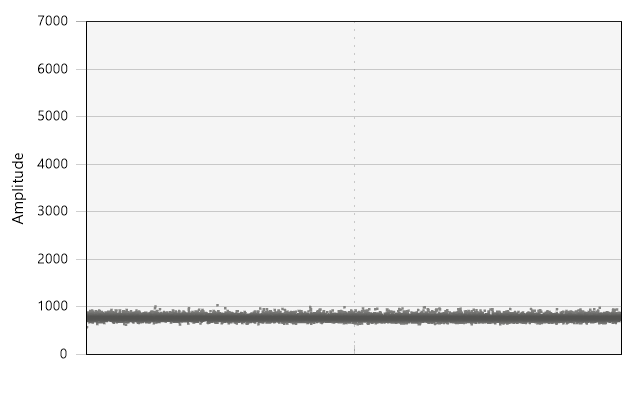
\includegraphics[scale = 0.6]{images/LG_negative}   
\end{subfigure}
\begin{subfigure}
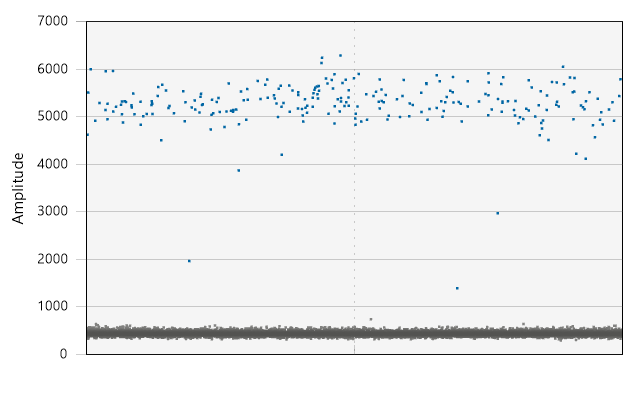
\includegraphics[scale = 0.6]{images/LG_positive}
\end{subfigure}
\caption{An example of amplitude plots for a positive control (bottom) and a negative control (top) from lake LG.}
\label{fig:amplitudes_controls}
\end{figure}

\newpage

\section{Acknowledgements}

I would like to thank Dr. Andrew Hoegh for the time spent helping me with this project and furthering my understanding of statistics in general. I would also like to thank Dr. Adam Sepulveda from the Northern Rocky Mountain Science Center for his collaboration and willingness to share his resources. Additionally, I would like to extend a thank you to Alison Watts from the University of New Hampshire for sharing her data. Finally, I would like to thank the entire Department of Mathematical Sciences Statistics faculty at Montana State University for helping me grow both as a statistician and as a student. 

\nocite{*}

\newpage
\section{References}

\begingroup
\renewcommand{\section}[2]{}%
\begin{flushleft}
\bibliographystyle{apalike}
%\bibliographystyle{acm}
%\bibliographystyle{abbrvnat}
%\bibliographystyle{unsrtnat}
%\bibliographystyle{ACM-Reference-Format}
\bibliography{bibliography}
\end{flushleft}
\endgroup

\newpage
\section{Appendix - R Code}

\singlespacing

\begin{small}

\begin{knitrout}
\definecolor{shadecolor}{rgb}{0.969, 0.969, 0.969}\color{fgcolor}\begin{kframe}
\begin{verbatim}
# packages used 
library(car)
library(dplyr)
library(tidyr)
library(dataRetrieval)
library(kableExtra)
library(ggplot2)
library(grid)
library(gridExtra)
library(tm)
library(readxl)
## library(devtools)
## devtools::install_github("StrattonCh/msocc")
library(msocc)
library(Rcppocc)


# load eDNA data
eDNA <- read.csv(
  "C:/Users/mwind/OneDrive/Writing Project_EXTRA/eDNA.csv")


# rename lakes
levels(eDNA$Lake) <- c("BOM", "LG", "MG")


# remove field blank samples
eDNA <- eDNA %>% 
  filter(Site != "tb")
eDNA$Site <- droplevels(eDNA$Site)


# reorder dates in chronological order
eDNA$Date.Collected <- factor(eDNA$Date.Collected,
                          levels = c("5/28/2019", 
                                     "7/8/2019", 
                                     "8/23/2019", 
                                     "9/25/2019",
                                     "10/21/2019"))

# vector of site names
Site.names <- unique(eDNA$Site)

# number of sites 
M <- length(Site.names)

# vector of lake names for each sample 
lake <- eDNA$Site %>% 
  as.character() %>%
  removeNumbers() %>%
  factor()

  
# generate table of 10 sample rows of eDNA data
set.seed(03142020)
knitr::kable(some(eDNA), 'latex', booktabs = T, linesep = "",
             caption = "\\label{tab:eDNA_data}
             10 sample rows of the eDNA data.", 
             align = 'c', row.names = F, 
             col.names = c("Lake", "Site", "Sample", "Date", 
                           "Water Temperature", "Concentration", 
                           "Positive Droplets")) %>%
  kable_styling(latex_options = 
                  c("scale_down", "hold_position"))


# BOM
eDNA %>% filter(Lake == "BOM") %>% summary


# LG
eDNA %>% filter(Lake == "LG") %>% summary


# MG
eDNA %>% filter(Lake == "MG") %>% summary


# number of samples with 0 positive droplets, by lake
eDNA %>% 
  group_by(Lake) %>%
  count(Positive.Droplets == 0)


# number of samples with (0, 3) positive droplets
eDNA %>% 
  group_by(Lake) %>%
  count(Positive.Droplets < 3  & Positive.Droplets > 0)


# number of samples with [3, 10] positive droplets
eDNA %>% 
  group_by(Lake) %>%
  count(Positive.Droplets > 3 & Positive.Droplets <= 10)


# overall summary of concentrations
summary(eDNA$Conc)

# mean concentration by site
eDNA %>%
  group_by(Site) %>%
  summarise(mean(Conc))


# summary at sample level 
## 3 or more positive droplets
eDNA$Detect3 <- rep(NA, nrow(eDNA))
for(i in 1:nrow(eDNA)){
  if(eDNA$Positive.Droplets[i] >= 3){
    eDNA$Detect3[i] <- 1
  } else {
      eDNA$Detect3[i] <- 0
      }
}


## number of postive samples in each site w/ threshold
site.detect3 <- eDNA %>% 
  group_by(Site) %>%
  summarise(sum(Detect3))


## total number of samples in each site 
count <- eDNA %>% 
  group_by(Site) %>% 
  count()


## proportions of positive samples in each site w/ threshold
cbind(Site = Site.names, site.detect3[, 2]/count[, 2])


## all positive droplets
eDNA$Detect <- rep(NA, nrow(eDNA))
for(i in 1:nrow(eDNA)){
  if(eDNA$Positive.Droplets[i] > 0){
    eDNA$Detect[i] <- 1
  } else {
      eDNA$Detect[i] <- 0
      }
}


site.detect <- eDNA %>% 
  group_by(Site) %>%
  summarise(sum(Detect))


eDNA.df2 <- data.frame(Site.names, 
                       site.detect[2]/count[2], 
                       site.detect3[2]/count[2])
names(eDNA.df2) <- c("Site", "Prop", "Prop3") 


# eDNA positive sample plot
prop.plot <- eDNA.df2 %>% 
  ggplot(aes(x = Site, 
             y = Prop)) + 
  geom_point() +
  labs(title = paste0('Proportion of Positive Samples by Site when 
      all Samples with Positive Droplets are Considered Positive'), 
       x = 'Site', 
       y = 'Proportion of Positive Samples') +
  ylim(c(0, 1)) +
  theme_bw() + 
  theme(title = element_text(size = 10),
        panel.border = element_blank(), 
        panel.grid.major = element_blank(),
        panel.grid.minor = element_blank(), 
        axis.line = element_line(colour = "black"))

# eDNA positive sample plot w/ threshold 
prop3.plot <- eDNA.df2 %>% 
  ggplot(aes(x = Site, 
             y = Prop3)) + 
  geom_point() +
  labs(title = paste0('Proportion of Positive Samples by Site when 
  the Threshold of 3 or more Positive Droplets is Used'), 
       x = 'Site', 
       y = 'Proportion of Positive Samples') +
  ylim(c(0, 1)) +
  theme_bw() + 
  theme(title = element_text(size = 10),
        panel.border = element_blank(), 
        panel.grid.major = element_blank(),
        panel.grid.minor = element_blank(), 
        axis.line = element_line(colour = "black"))

# plot positive sample plots w/ and w/o threshold 
# vertically stacked
grid.arrange(prop.plot, prop3.plot, nrow = 2)


# replace missing water temps from lake BOM with 14C
eDNA$Water.Temp <- replace(eDNA$Water.Temp, 
                           is.na(eDNA$Water.Temp), 14)


# denote which water temperatures were estimated
est.water.temp <- as.numeric(eDNA$Date.Collected == "10/21/2019" 
                             & eDNA$Lake == "BOM")

eDNA.df2 <- data.frame(eDNA, 
                       Est.Water.Temp = factor(est.water.temp), 
                       lake = lake)

levels(eDNA.df2$Est.Water.Temp) <- c("Observed", "Estimated")


# eDNA water temperature plot
eDNA.df2 %>% 
  ggplot(aes(x = Site, 
             y = Water.Temp, 
             colour = Date.Collected)) + 
  labs(title = 'Water Temperature by Site', 
       x = 'Site', 
       y = expression(paste('Water Temperature (', degree,
                            'C)')), 
       color = 'Date') +
  geom_point(aes(shape = Est.Water.Temp)) + 
  scale_colour_manual(values = date.cols) + 
  scale_shape_manual(values = c(16, 8)) + 
  theme_bw() +
  guides(shape = guide_legend(title = NULL)) + 
  theme(title = element_text(size = 10),
        panel.border = element_blank(), 
        panel.grid.major = element_blank(),
        panel.grid.minor = element_blank(), 
        axis.line = element_line(colour = "black"), 
        legend.position = 'bottom', 
        legend.box = 'vertical')


# format data for use in PGocc4 function
## number of samples per sites
J <- rep(0, M)

for(j in 1:length(J)){
  for(i in 1:nrow(eDNA)){
    if(eDNA$Site[i] == Site.names[j]){
      J[j] <- J[j] + 1
    }
  }
}


## vector of the sample number in each site 
samp <- matrix(NA, nrow = M, ncol = max(J))

for(i in 1:M){
  if(J[i] == ncol(samp)){
    samp[i, ] <- seq(1:J[i])
  } else {
    samp[i, 1:J[i]] <- seq(1:J[i])
  }
}

samp <- na.omit(as.vector(t(samp)))


## detection/non-detection matrix
y <- matrix(NA, nrow = M, ncol = max(J))

for(i in 1:M){
  for(k in 1:nrow(eDNA)){
    if(eDNA$Site[k] == Site.names[i] & eDNA$Detect3[k] == 1){
      y[i, samp[k]] <- 1
    } else if(eDNA$Site[k] == Site.names[i] & eDNA$Detect3[k] == 0){
      y[i, samp[k]] <- 0
      }
  }
}  

y <- matrix(as.integer(y), nrow = M, ncol = max(J))


## site level covariates
X <- data.frame(Site.names)
names(X) <- "site"
X[, 2] <- X$site %>%
  as.character() %>%
  removeNumbers() %>%
  factor()

X <- as.matrix(X)

colnames(X)[2] <- "lake"


## sample level covariates
### water temperature
W1 <- matrix(NA, nrow = M, ncol = max(J))

for(i in 1:M){
  if(J[i] == ncol(W1)){
    W1[i, ] <- eDNA$Water.Temp[eDNA$Site == Site.names[i]]
  } else {
    W1[i, 1:J[i]] <- eDNA$Water.Temp[eDNA$Site == Site.names[i]]
    }
}

### date
W2 <- data.frame(matrix(NA, nrow = M, ncol = max(J)))

for(i in 1:M){
  if(J[i] == ncol(W2)){
    W2[i, ] <- eDNA$Date.Collected[eDNA$Site == Site.names[i]]
  } else {
    W2[i, 1:J[i]] <- eDNA$Date.Collected[eDNA$Site == Site.names[i]]
    }
}

W2 <- as.matrix(W2)

### site 
W3 <- data.frame(matrix(NA, nrow = M, ncol = max(J)))

for(i in 1:M){
  if(J[i] == ncol(W3)){
    W3[i, ] <- eDNA$Site[eDNA$Site == Site.names[i]]
  } else {
    W3[i, 1:J[i]] <- eDNA$Site[eDNA$Site == Site.names[i]]
    }
}

W3 <- as.matrix(W3)

### lake
W4 <- data.frame(matrix(NA, nrow = M, ncol = max(J)))

for(i in 1:M){
  if(J[i] == ncol(W4)){
    W4[i, ] <- rep(X[i, 2], ncol(W4))
  } else {
    W4[i, 1:J[i]] <- rep(X[i, 2], J[i])
  }
}

W4 <- as.matrix(W4)

## list of sample covariates
W <- list(W1 = W1, W2 = W2, W3 = W3, W4 = W4)


# merge for use in PGocc4
data <- vb_Designs(W = W, X = X, y = y)


# function to summarize the alpha, beta, p, and psi estimates 
post_summary <- function(parameter.matrix, param, plot = T){
  mean <- apply(parameter.matrix, 1, mean)
  median <- apply(parameter.matrix, 1, median)
  min <- apply(parameter.matrix, 1, min)
  lwr <- apply(parameter.matrix, 1, quantile, probs = 0.025)
  upr <- apply(parameter.matrix, 1, quantile, probs = 0.975)
  max <- apply(parameter.matrix, 1, max)
  out <- cbind("mean" = mean, 
               "median" = median, 
               "min" = min, 
               "2.5%" = lwr , 
               "97.5%" = upr, 
               "max" = max)
  if(missing(param)){
    out <- out
  } else if(param == "psi"){
    out <- cbind.data.frame(out, 
                            rownames = Site.names)
  } else if(param == "p"){
    out <- cbind.data.frame(Site = eDNA$Site, 
                            Sample = samp, 
                            out)
  } else if(param == "alpha"){
    rownames(out) <- paste("alpha", 0:(nrow(out) - 1))
  } else if(param == "beta"){
    rownames(out) <- paste("beta", 0:(nrow(out) - 1))
  }
  if(plot == T){
    tr.plot <- list()
    for(i in 1:nrow(parameter.matrix)){
      df <- data.frame(param = parameter.matrix[i, ], 
                       iter = 1:ncol(parameter.matrix))
      tr.plot[[i]] <- ggplot(df, aes(x = iter, y = param)) + 
        geom_path() + 
        xlab("Post Burn-in Iterations") + 
        ylab(rownames(out)[i]) + 
        theme_bw() + 
          theme(title = element_text(size = 10),
                panel.border = element_blank(), 
                panel.grid.major = element_blank(),
                panel.grid.minor = element_blank(), 
                axis.line = element_line(colour = "black"))
    }
    if (missing(param)){
      print(grid.arrange(grobs = tr.plot, ncol = 2))
    } else if (param == 'beta'){
      print(grid.arrange(grobs = tr.plot, ncol = 2, 
            top = textGrob(expression(paste("Trace Plots of the ", 
                                            beta, "'s")))))
    } else if (param == 'alpha'){
      print(grid.arrange(grobs = tr.plot, ncol = 2, 
            top = textGrob(expression(paste("Trace Plots of the ", 
                                            alpha, "'s")))))
    } else if (param == 'p') {
      print(grid.arrange(grobs = tr.plot, ncol = 2, 
            top = textGrob("Trace Plots of the p's")))
    } else if (param == 'psi'){
      print(grid.arrange(grobs = tr.plot, ncol = 2, 
            top = textGrob(expression(paste("Trace Plots of the ", 
                                            psi, "'s")))))
    }
  } 
  return(out)
}


# function to generate nice looking plots
# of credible intervals for p and psi
cred_plot <- function(post_summary_out, parameter){
  df <- data.frame(post_summary_out)
  if(nrow(df) == 12){
    rownames(df) <- Site.names
  } 
  if(parameter == "psi"){
    cred.plot <- ggplot(df, aes(x = rownames(df), y = mean)) + 
      geom_point() + 
      xlab("") + 
      geom_errorbar(aes(ymax = X97.5., ymin = X2.5.), width = 0) + 
      theme_bw() + 
      theme(title = element_text(size = 10),
            panel.border = element_blank(), 
            panel.grid.major = element_blank(),
            panel.grid.minor = element_blank(), 
            axis.line = element_line(colour = "black"), 
            axis.text.x = element_text(angle = 45, hjust = 1)) +
      ylab(expression(paste("Estimated ", psi))) 
  } else if(parameter == "p"){
    cred.plot <- ggplot(df, aes(x = eDNA$Date.Collected, y = mean)) + 
      geom_point() + 
      xlab("") + 
      geom_errorbar(aes(ymax = X97.5., ymin = X2.5.), width = 0) + 
      theme_bw() + 
      theme(title = element_text(size = 10),
            panel.border = element_blank(), 
            panel.grid.major = element_blank(),
            panel.grid.minor = element_blank(), 
            axis.line = element_line(colour = "black"), 
            axis.text.x = element_text(angle = 45, hjust = 1)) + 
      ylab("Estimated p") + 
      facet_wrap(~Site) 
  }
  print(cred.plot)
}
  

# model psi ~ lake, p ~ water.temp

# Priors 

## beta ~ MVN(0, 100^2I)
### prior mean for beta
beta_m <- matrix(0, nrow = 3, ncol = 1) 
#### prior precision for beta
sigma_inv_beta <- diag(nrow(beta_m))/10000 

## alpha ~ MVN(0, 100^2I)
### prior mean for alpha
alpha_m <- matrix(0, nrow = 2, ncol = 1) 
### prior precision for alpha
sigma_inv_alpha <- diag(nrow(alpha_m))/10000 


# fit the model 
set.seed(04172020)
m5 <- PGocc4(formula = V1 ~ lake ~ as.numeric(W1), 
             design_mats = data, 
             ndraws = 50000, 
             alpha_m = alpha_m, 
             beta_m = beta_m, 
             sigma_inv_alpha_p = sigma_inv_alpha, 
             sigma_inv_beta_p = sigma_inv_beta, 
             percent_burn_in = 1/10)


# extract beta estimates from model output
m5.beta <- m5$beta

# posterior summary and trace plots of beta estimates
m5.beta.sum <- post_summary(m5.beta, 'beta')


# extract alpha estimates from model output
m5.alpha <- m5$alpha

# posterior summary and trace plots of alpha estimates
m5.alpha.sum <- post_summary(m5.alpha, 'alpha')


# table of beta estimates
m5.beta.sum
# table of alpha estimates
m5.alpha.sum
# summary of psi
## calculate estimates of psi from estimates of beta
m5.psi.mcmc <- exp(model.matrix(~data$X$lake) %*% m5.beta)/
  (1 + exp(model.matrix(~data$X$lake) %*% m5.beta))

## summary of psi
m5.psi.sum <- post_summary(m5.psi.mcmc, 'psi', plot = F)
m5.psi.sum

# credible interval plot for psi
cred_plot(m5.psi.sum, 'psi')


# summary of p
## calculate estimates of p from estimates of alpha
m5.p.mcmc <- exp(model.matrix(~as.numeric(data$W$W1)) %*% m5.alpha)/
  (1 + exp(model.matrix(~as.numeric(data$W$W1)) %*% m5.alpha))

## summary of p
m5.p.sum <- post_summary(m5.p.mcmc, 'p', plot = F)
m5.p.sum 

## credible interval plot for p
cred_plot(m5.p.sum, 'p')


# table of p* for each site
names(m5.p.sum)[6:7] <- c("lwr", "upr")

m5.p.sum

tmp <- rep(NA, M)
p.star <- rep(NA, M)

m5.p.sum %>%
  group_by(Site) %>% 
  summarise(p.star.lwr = 1 - prod(1 - lwr), 
            p.star.upr = 1 - prod(1 - upr)) 
\end{verbatim}
\end{kframe}
\end{knitrout}

\end{small}

\lstset{
	basicstyle=\ttfamily\scriptsize,
	columns = fullflexible,
	frame = single,
	breaklines = true,
	postbreak = \mbox{\textcolor{red}{$\hookrightarrow$}\space},
	keepspaces = TRUE,
}
%\begin{lstlisting}
%\end{lstlisting}
\end{document}
              
